\documentclass[
aip,
jcp,
%preprint,
reprint,
]{revtex4-1}
%
\usepackage[hyperindex,breaklinks,hidelinks,colorlinks,citecolor=blue]{hyperref}
\usepackage{amsmath, amsthm, amssymb}    
\usepackage{float}
%
\usepackage{graphicx}
\DeclareGraphicsExtensions{.pdf,.eps,.png}
\graphicspath{{Figures/}}
\usepackage[outdir=Figures/]{epstopdf}
%
\usepackage{natmove}
%
%\usepackage{adjustbox}
%
%\usepackage{mathtools}
%\mathtoolsset{showonlyrefs}
%
\DeclareMathOperator\arctanh{arctanh}
\DeclareMathOperator\arcsinh{arcsinh}
\DeclareMathOperator\sech{sech}
%
\newcommand{\mt}[1]{\boldsymbol{\mathbf{#1}}}          % matrix symbol
\newcommand{\vt}[1]{\boldsymbol{\mathbf{#1}}}          % vector symbol
\newcommand{\tr}[1]{#1^\text{t}}                       % transposition
\newcommand{\diff}[2]{\frac{\partial #2}{\partial #1}} % derivative
\newcommand{\avg}[1]{\overline{#1}}                    % average
%\newcommand{\Liu}[1]{\mathcal{L}_{#1}}                 % Liouville operator
\newcommand{\Liu}{\mathcal{L}}
\newcommand{\Ham}[1]{{\mathcal H}_\mathrm{#1}}         % Hamiltonian
\newcommand{\nn}{n}

\begin{document}

\author{Charlles R. A. Abreu}
\email{abreu@eq.ufrj.br}
\affiliation{Chemical Engineering Department, Escola de Qu\'imica, Universidade Federal do Rio de Janeiro, Rio de Janeiro, RJ 21941-909, Brazil}
\affiliation{Department of Chemistry, New York University, New York, New York 10003, USA}

\author{Mark E. Tuckerman}
\email{marktuckerman@nyu.edu}
\affiliation{Department of Chemistry, New York University, New York, New York 10003, USA}
\affiliation{Courant Institute of Mathematical Sciences, New York University, New York, New York 10012, USA}
\affiliation{NYU-ECNU Center for Computational Chemistry at NYU Shanghai, Shanghai 200062, China}

\title{Solvation Free-Energy Calculations with Very Large Time Steps}

\keywords{molecular dynamics; multiple time-stepping; resonance}

\date{\today}

\maketitle

\section{Methods}
\label{sec:methods}

\subsection{Simulation Method}
\label{sec: simulation method}

In all cases, the SIN(R) method \cite{Leimkuhler_2013} was employed with a single thermostat acting on each degree of freedom (i.e. $L = 1$).
The employed friction coefficient was $\gamma = 0.1~\mathrm{fs^{-1}}$ and the characteristic time scale chosen for the thermostats was $\tau = 10~\mathrm{fs}$ (with the inertial parameters of the thermostats computed as $Q_1 = Q_2 = kT \tau^2$, as usual).

The equations of motion were integrated by using a multiple time scale extension of the \textit{middle scheme} \cite{Zhang_2017}.
This means that all thermostat-related variables are integrated in the innermost loop, that is, with the same time step as the fastest forces in the system.
Moreover, in the Trotter-Suzuki splitting of the classical propagator, the thermostat-related operator goes right in the middle, between atomic coordinate moves.

The forces were split according to the RESPA-2 scheme \cite{Zhou_2001, Morrone_2010, Leimkuhler_2013} with three separate time scales.
The fastest forces include bonded interactions such as bond stretching, bending, and torsion.
Included in the middle time scale are the short-range contribution of van der Waals and Coulomb interactions, with an applied cut-off of $8~\mathrm{\AA}$ and a smooth decay to zero starting from $5~\mathrm{\AA}$.
Finally, the slowest forces comprise the long-range contributions of these non-bonded interactions, including the reciprocal-space part of the electrostatic potential (with the proper discount of short-range terms).

For this splitting scheme to work with very large time steps, it is essential to apply the switching function directly to the computed forces, rather than to the potential energy.
This observation seemingly contradicts an assertion by \citeauthor{Morrone_2010} \cite{Morrone_2010} that both types of switching lead to similarly smooth trajectories.
However, the contradiction is only apparent because in such reference the feasible size of a time step was limited by the emergence of resonance artifacts.

\subsection{Free Energy Calculation}
\label{sec:free energy calculation}

Free energies of a given system were computed by simulating it at independent constant-$NVT$ equilibrium states and combining all the sampled configurations together.
The Multistate Bennett Acceptance Ratio (MBAR) estimator \cite{Kong_2003, Shirts_2008} for the free energies of $m$ states consists in a set of self-consistent equations given by
\begin{equation}
\label{eq:mbar free energy estimator}
\hat f_i = -\ln \sum_{k=1}^n \frac{e^{-u_i(\vt r_k)}}{\sum_{j=1}^m n_j e^{-u_j(\vt r_k) + \hat f_j}},
\end{equation}
where $n_j$ is the number of uncorrelated configurations sampled at state $j$, $n = \sum_{j=1}^m n_j$ is the size of the pooled sample obtained from all states, and $u_i(\vt r_k)$ is the reduced potential of configuration $k$ at state $i$.
In the case of our alchemical free energy calculations, we have
\begin{equation}
u_i(\vt r) = \frac{U_\mathrm{ab}(\vt r, \lambda_i)}{k_B T},
\end{equation}
where $U_\mathrm{ab}(\vt r, \lambda)$ is the potential energy concerning the solute-solvent interactions, which are affected by the value of a coupling parameter $\lambda$.
In our approach, the solute-solute ($U_\mathrm{aa}$) and solvent-solvent ($U_\mathrm{bb}$) interactions are unaffected by such parameter.
This makes possible to have the solute simply decoupled from the solvent instead of annihilated completely.
Hence, what we denominate as solvation free energy in the forthcoming sections is in fact the solute-coupling free energy difference estimated as $\Delta F = k_B T ({\hat f}_{\lambda=1} - {\hat f}_{\lambda=0})$.

\section{Results}
\label{sec:results}

%\subsection{Chemical Potential of Lennard-Jones Fluid}
%\label{sec:lennard-jones chemical potential}
%
%In this section, we present results concerning the chemical potential of a Lennard-Jones fluid, i.e. the solvation free energy of a single particle in such fluid.
%Although we employed parameters determined from experimental data for argon \cite{White_1999}, the analysis is evidently prone to a corresponding-states analogy.
%The parameters we employed are $m = 39.948~\mathrm{Da}$, $\sigma = 3.405~\mathrm{\AA}$, and $\epsilon/k_B = 125.2~\mathrm{K}$, where $k_B$ is the Boltzmann constant.
%A truncated/smoothed Lennard-Jones model was used, in which the standard potential energy $V(r) = 4\epsilon[(\sigma/r)^{12}-(\sigma/r)^6]$ is multiplied by
%\begin{equation*}
%%f(z) = \begin{cases}
%%1 & z < 0 \\
%%1 - 10 z^3 + 15 z^4 - 6 z^5 & 0 \leq z \leq 1 \\
%%0 & z > 1
%%\end{cases},
%f(z) = \theta(-z) + \sqcap(z) (1 - 10 z^3 + 15 z^4 - 6 z^5),
%\end{equation*}
%where $z = \frac{r+\delta r-r_c}{\delta r}$.
%The values we specified for the cut-off distance and the healing length were, respectively, $r_c = 10~\mathrm{\AA}$ and $\delta r = 1~\mathrm{\AA}$.
%In all simulations, the total number of particles (including the one affected by the coupling parameter $\lambda$) was $250$.
%The simulation box was a cubic one with periodic boundary conditions and side length $L = 22.734~\mathrm{\AA}$, resulting in a reduced density $\rho^\ast = 0.84$ when $\lambda = 1$.
%The temperature in all simulations was $T = 300~\mathrm{K}$, yielding a reduced temperature $T^\ast = 2.396$.
%
%According to the Lennard-Jones equations of state by \citeauthor{Johnson_1993} \cite{Johnson_1993}, which is supposed to reproduce a full (as opposed to truncated and smoothed) potential, the chemical potential at $\rho^\ast = 0.84$ and $T^\ast = 2.396$ is $9.20~\mathrm{kJ/mol}$.
%
%
%
%
%We executed equilibrium NVT-ensemble simulations at 21 evenly spaced values of $\lambda$ between $0$ and $1$ by using a Langevin thermostat with the BAOAB integration method \cite{Leimkuhler_2012, Leimkuhler_2013}.
%The time step size was $3~\mathrm{fs}$.
%After $300~\mathrm{ps}$ of equilibration at a given $\lambda_i$, information was collected during $3~\mathrm{ns}$, including the derivative of the potential energy with respect with $\lambda$ evaluated at $\lambda_i$, as well as the set of potential energies evaluated at $\lambda_j$ for all $j \in [1,21]$.
%This allows us to compute the free energy profile using both TI and MBAR.
%
%
\subsection{Hydration Free Energy of a Single Lennard-Jones Particle}
\label{sec:hydration free energy}

In this section we report an exploratory study of the hydration of a very simple solute, which is a single, electrically neutral Lennard-Jones particle.
For this, we used the TraPPE united-atom model for methane \cite{Siepmann_1998}.
It has been shown to reproduce experimentally determined properties of pure methane in a wide range of thermodynamic conditions \cite{Aimoli_2014}.
The Lennard-Jones parameters for this model molecule are $\sigma = 3.730~\mathrm{\AA}$ and $\epsilon/k_B = 148.0~\mathrm{K}$.
For the solvent, we adopted the parameters of the fully-flexible q-SPC-Fw model \cite{Paesani_2006}.
A truncated/smoothed Lennard-Jones model was used, in which the forces the standard potential $V_\mathrm{LJ}(r) = 4\epsilon[(\sigma/r)^{12}-(\sigma/r)^6]$ is multiplied by $f_5(\frac{r+\delta r-r_c}{\delta r})$, where $r_c$ is the cut-off distance, $\delta r$ is a healing length (along which the potential smoothly decays to zero), and $f_5(z)$ is a 5th-degree switch given by
\begin{equation}
\label{eq:swithing function}
f_5(z) = \begin{cases}
1 & z < 0 \\
1 - 10 z^3 + 15 z^4 - 6 z^5 & 0 \leq z \leq 1 \\
0 & z > 1
\end{cases}.
%f(z) = \theta(-z) + \sqcap(z) (1 - 10 z^3 + 15 z^4 - 6 z^5),
\end{equation}

The interactions were evaluated by considering $r_c = 12~\mathrm{\AA}$ and $\delta r = 1~\mathrm{\AA}$, along with standard long-range corrections.
They take place in a cubic simulation box with side length $L$ and periodic boundary conditions.
Electrostatic interactions were computed via Ewald sum.
The same cut-off distance $r_c$ was adopted for the real-space part, with a damping parameter $\alpha = {\sqrt{-\ln(2\delta)}}/{r_c}$, where $\delta = 10^{-5}$.
The reciprocal-space part was solved by using the Particle-Mesh Ewald (PME) method \cite{Darden_1993} with $n_{\rm mesh} \approx \frac{2}{3} \alpha L \delta^{-1/5}$.

In this study, we simulated $1$ methane molecule and $499$ water molecules.
With the solute in its fully-coupled state, the system was equilibrated at $298.15~\mathrm{K}$ and $1~\mathrm{atm}$ during $2~\mathrm{ns}$.
For this, we employed a Langevin integrator with time step size of $1~\mathrm{fs}$ and a Monte Carlo barostat \cite{Chow_1995, Aqvist_2004} acting at every 20 steps, with the maximum allowable volume change adjusted to yield an acceptance rate of about 50\%.
The average box volume during the final half of the equilibration was then adopted in the subsequent NVT simulations.

The box side length determined as described above was $L = 24.47~\mathrm{\AA}$, resulting in a density $\rho = 1.0206~\mathrm{g/cm^3}$.
In the solvation free-energy calculations, the simulated temperature was also $298.15~\mathrm{K}$.
All solvent-solvent van der Waals interactions were computed using the standard Lennard-Jones model.
For the solute-solvent interactions, however, we employed two different strategies to make it depend continuously on a coupling parameter $\lambda$, so that the full Lennard-Jones potential takes place when $\lambda = 1$, but no interaction occurs at all when $\lambda = 0$.

The first strategy consists in a simple scaling by a coupling function $g(\lambda)$ that increases monotonically from $g(0) = 0$ to $g(1) = 1$.
Therefore, the solute-solvent interaction potential is given by
\begin{equation*}
V_\mathrm{scaling}(r,\lambda) = 4 g(\lambda) \epsilon \left[\left(\frac{\sigma}{r}\right)^{12} - \left(\frac{\sigma}{r}\right)^6\right].
\end{equation*}

It is worth noting that, when discrete states are sampled independently in order to yield a free energy estimate, it would be equivalent as a state-selection strategy to 1) employ different coupling functions and a fixed set of supporting points or 2) employ a single coupling function and distinct sets of supporting points.
For instance, if the traditional choice of a simple linear coupling is made, meaning that $g(\lambda) = \lambda$, then it becomes necessary to concentrate many of the sampled states at very small values of $\lambda$.
Here we prefer to spread the points uniformly along the interval $\lambda \in [0, 1]$ and try different options for $g(\lambda)$.
One of the tested options was  $g(\lambda) = \lambda-\frac{\sin(2\pi\lambda)}{2\pi}$, a function which \citeauthor{Abrams_2006} \cite{Abrams_2006} recommended for solvation free energy calculations with an alternative approach in which $\lambda$ becomes a dynamical coordinate along with the atomic positions.
This is very closely related to using $g(\lambda) = 1 - f_5(\lambda)$, where $f_5$ is the same switching function defined in Eq.~\eqref{eq:swithing function}.
One can easily grasp such a close relationship in Fig.~\ref{fig:coupling functions}.
These functions have an interesting feature in common.
Their first- and second-order derivatives are both null at the extremes $\lambda = 0$ and $\lambda=1$.
When a uniform grid of $\lambda$'s is used, they tend to concentrate more values of $g$ in the proximities of $0$ and $1$ than in the middle of the interval.
Finally, after preliminary tests, we chose to employ another 5th-degree function whose first-, second-, and third-order derivatives are all null at $\lambda=0$, thus resulting in an asymmetrically high concentration of points with $g \to 0$, as it is needed for the problem in question.
Such choice is
\begin{equation}
g(\lambda) = \lambda^4 (5 - 4 \lambda).
\end{equation}

\begin{figure}
	\centering
	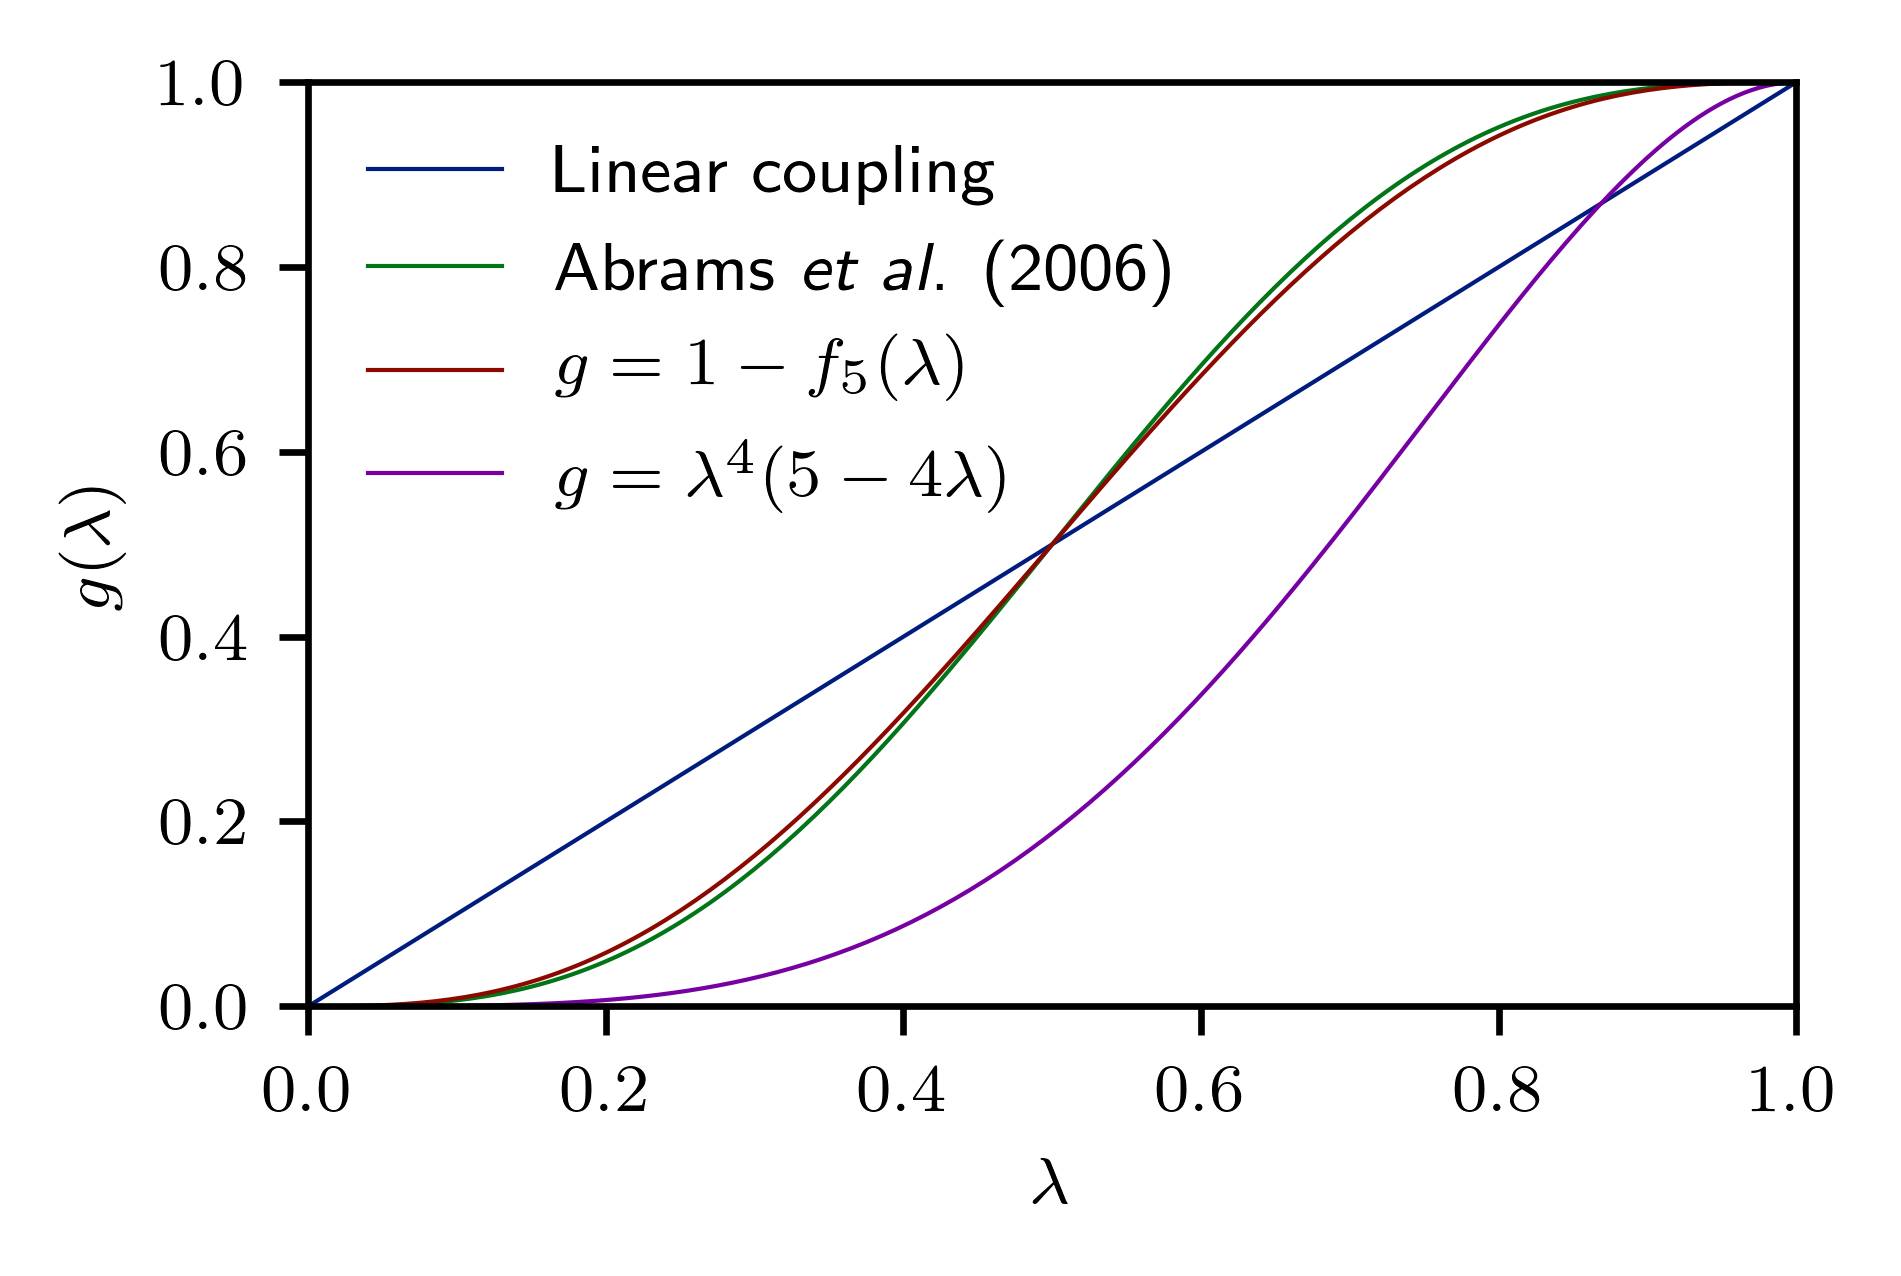
\includegraphics{coupling_functions}
	\caption{Possible coupling functions to be used for the scaling approach.}
	\label{fig:coupling functions}
\end{figure}

The second coupling strategy we employed consists in using an instance of the so-called softcore potential \cite{Beutler_1994} given by
\begin{equation*}
V_\mathrm{softcore}(r,\lambda) = 4 \lambda \epsilon \left[\left(\frac{\sigma^6}{r^6 + \frac{1-\lambda}{2}\sigma^6}\right)^2 - \frac{\sigma^6}{r^6 + \frac{1-\lambda}{2}\sigma^6}\right].
\end{equation*}

(Compare the advantages and drawbacks of both strategies....)

With each one of the coupling strategies, long simulations of carried out independently at 21 regularly spaced values of $\lambda$ between $0$ and $1$.
Each simulation consisted of $4.5~\mathrm{ns}$ of total simulated time, with the samples being taken from the final $3.6~\mathrm{ns}$.
The statistical inefficiency is usually very high when we deal exclusively with the interactions of a single solute molecule with the surrounding solvent.
By using an integrated autocorrelation function approach, \cite{Chodera_2007} we estimated that the correlation time of the full solute-solvent potential energy, $U_{ab}(\vt r, 1)$, can be as large as $2~\mathrm{ps}$ at some intermediate $\lambda$ states.
In order to have uncorrelated samples so that uncertainties can be properly estimated from the MBAR analysis, we adopted a sampling interval of $2.25~\mathrm{ps}$ for all simulations.
In this way, we ended up with $1600$ configurations sampled at each state, adding up to $33600$ configurations in the pooled multistate sample.

For each coupling strategy, we repeated the procedure several times, each one with a different size for the external time step of the SIN(R) simulation method.
The employed values for $\Delta t$ were $1~\mathrm{fs}$, $3~\mathrm{fs}$, $6~\mathrm{fs}$, $9~\mathrm{fs}$, $15~\mathrm{fs}$, $30~\mathrm{fs}$, $45~\mathrm{fs}$, and $90~\mathrm{fs}$.
In all cases, the step size of the innermost integration loop (shortest time scale) was $0.5~\mathrm{fs}$.
A force splitting with only two time scales (bonded interactions in the shortest scale and full non-bonded interactions in the longest one) were considered for the two first cases, that is, with $\Delta t = 1~\mathrm{fs}$, and $\Delta t = 3~\mathrm{fs}$.
In all other cases, the three-scale splitting described in Sec.~\ref{sec: simulation method} was applied with an intermediate time step size of $3~\mathrm{fs}$.

\begin{figure}
	\centering
	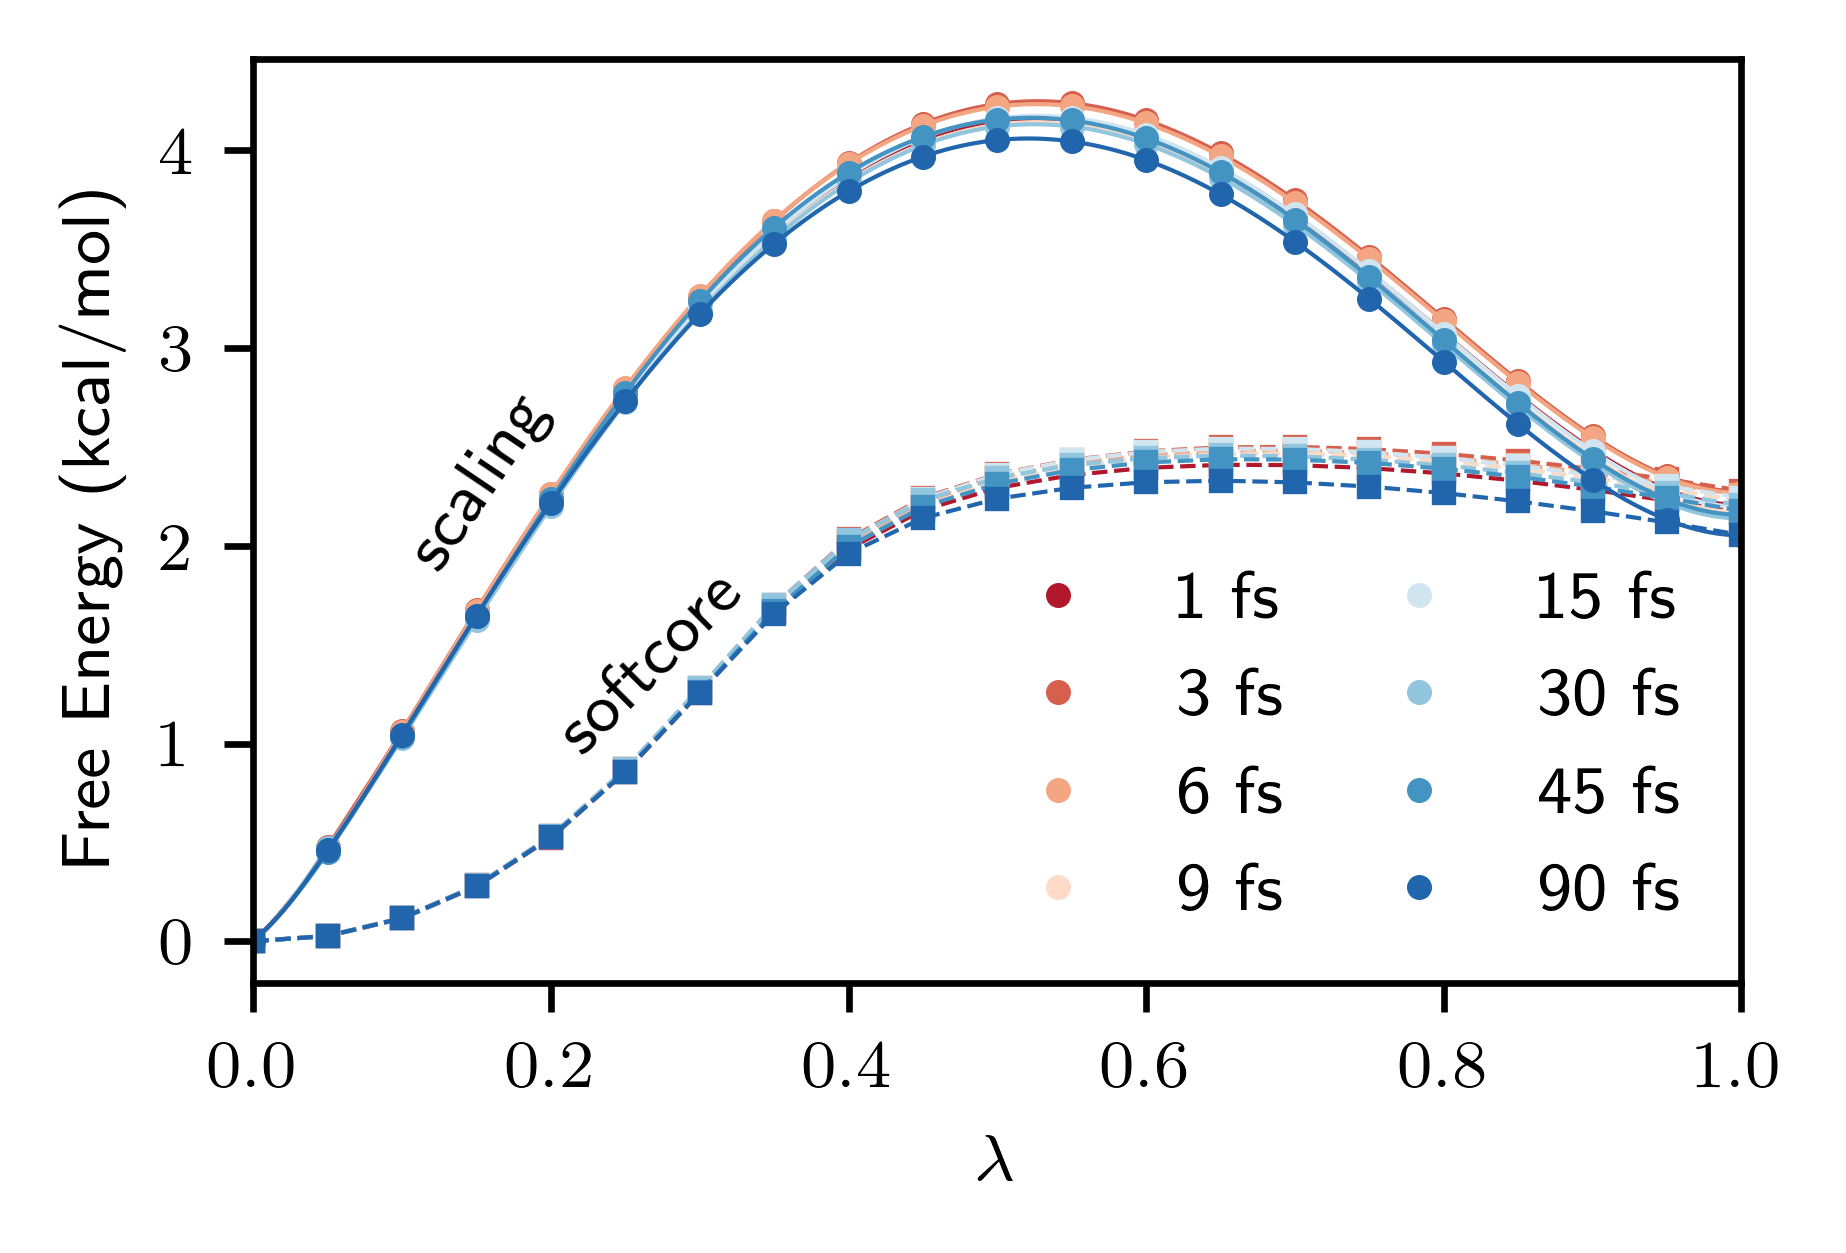
\includegraphics{trappe_methane_vdw_free_energy_profiles}
	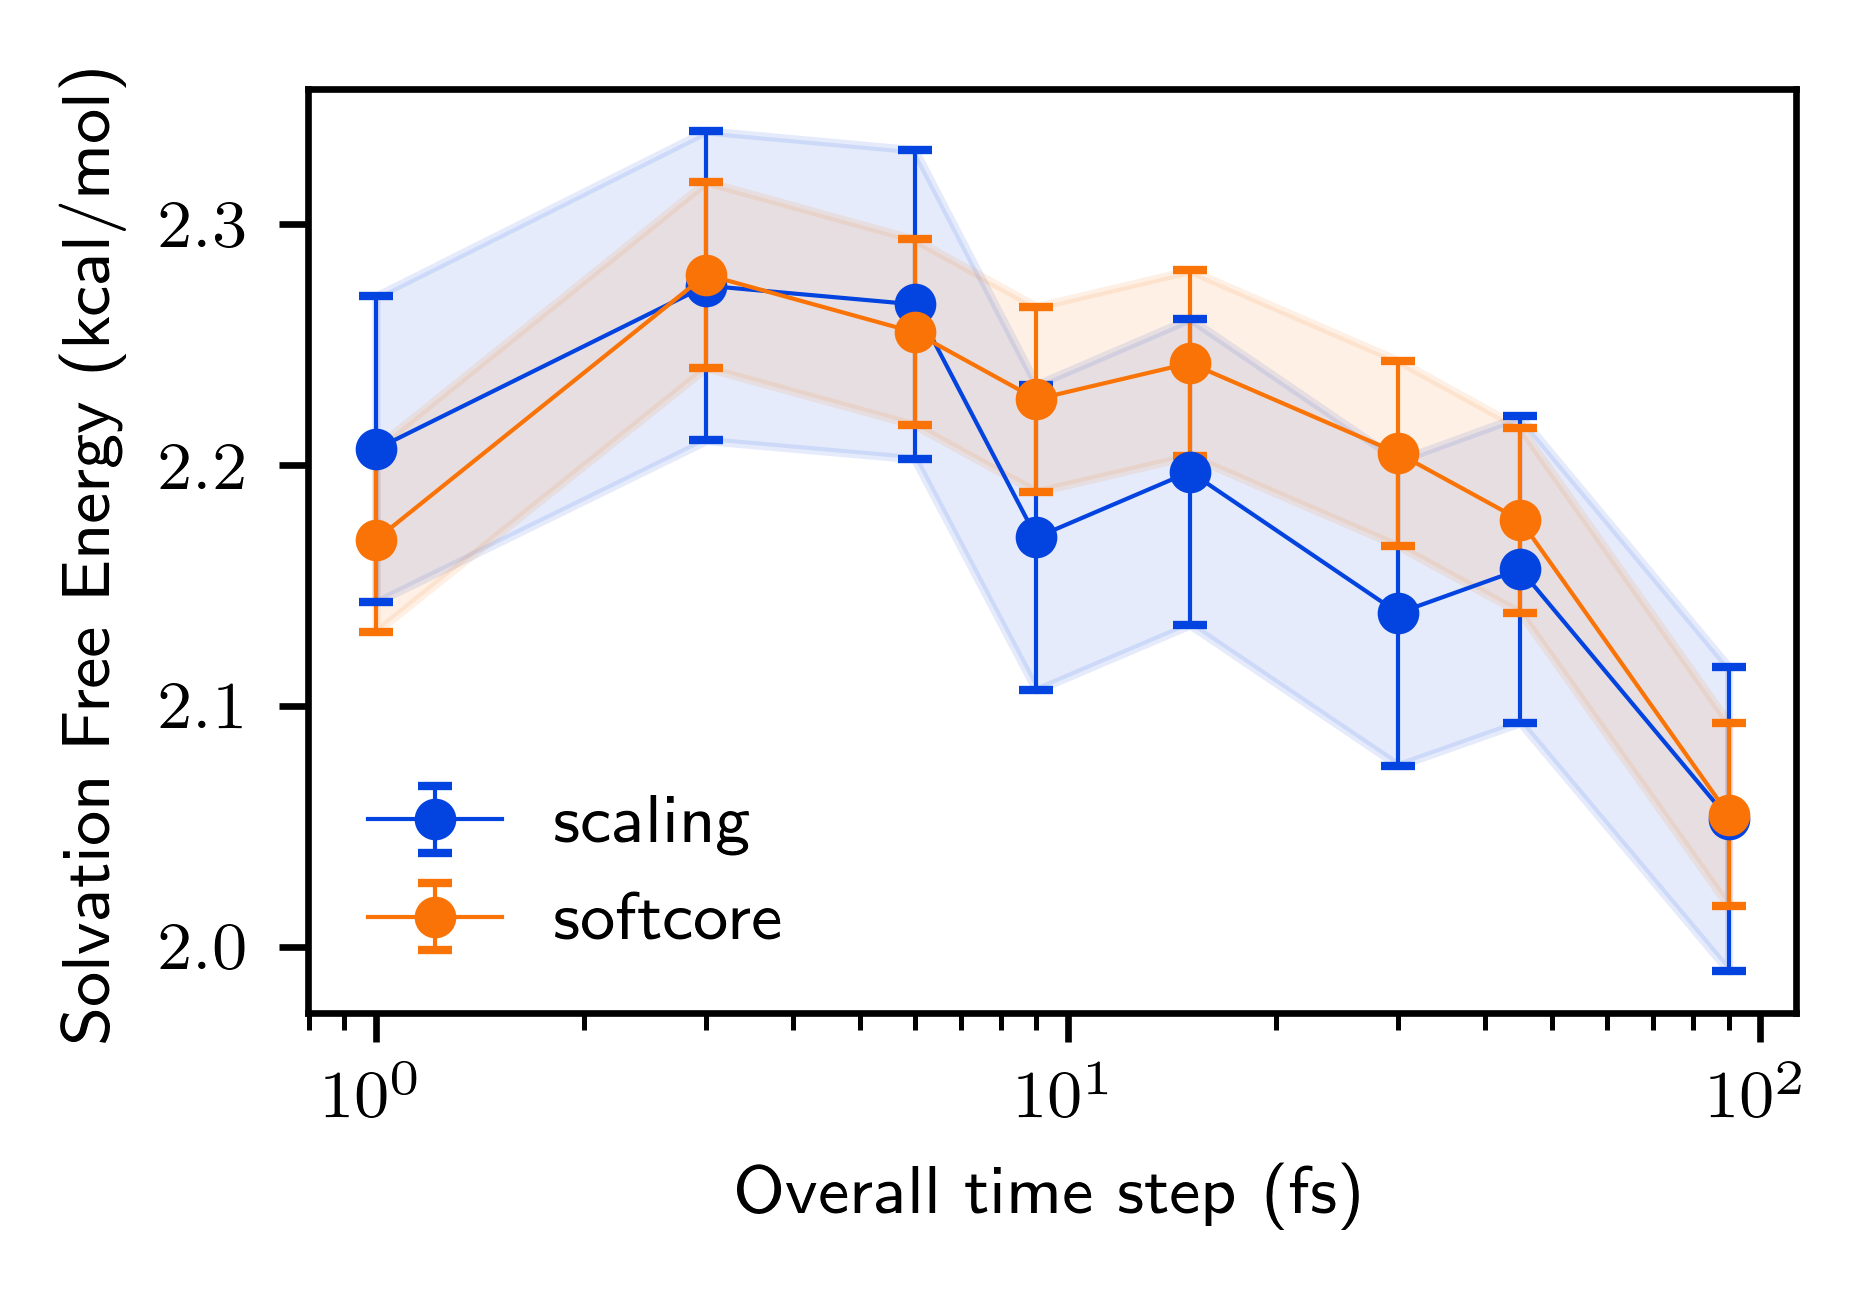
\includegraphics{trappe_methane_vdw_free_energies}
	\caption{TraPPE-UA Methane Free Energy.}
	\label{fig:methane free energy}
\end{figure}

\subsection{Hydration Free Energy of Charged Solutes}

In the case of charged molecules, we divided the solvation free energy calculation into two parts.
In the first part, the coupling/uncoupling of the solute and solvent is done by disregarding the electrostatic potential between them.
Therefore, only the van der Waals contribution is considered for the solute-solvent interactions, with its intensity tuned by a coupling parameter $\lambda_\mathrm{vdW}$.
Note that the intramolecular interactions are always present, including the electrostatic ones.
The calculation of $\Delta F_\mathrm{vdW}$ in this first part is done exactly as described in the preceding section for a single Lennard-Jones particle.
In the second part, with the van der Waals contribution of the solute-solvent potential in its fully coupled state, we proceed with the coupling/uncoupling of their electrostatic interactions.
This is done by a linear coupling such as
\begin{equation*}
V_\mathrm{coulomb}(r_{ij},\lambda_\mathrm{coul}) = \frac{\lambda_\mathrm{coul}}{4 \pi \epsilon_0} \frac{q_i q_j}{r_{ij}},
\end{equation*}
where $r_{ij}$ is the distance between a solute atom $i$ and a solvent atom $j$, whose electric charges are $q_i$ and $q_j$, respectively.
In practice, an Ewald-sum splitting is used instead of the the simple Coulomb form as above.
By simulating independent states with different values of $\lambda_\mathrm{coul} \in [0, 1]$, we can apply MBAR to compute the total free energy difference $\Delta F_\mathrm{coul}$.
Finally, the solvation free energy of a charged solute molecule is calculated as
\begin{equation}
\Delta F = \Delta F_\mathrm{vdW} + \Delta F_\mathrm{coul}.
\end{equation}

Four different polar molecules of distinct sizes and charge distributions, namely methanol, phenol, 1,4-dioxane, and dibenzo-p-dioxin, were considered in the present study.
Their structures can be seen in Fig.~\ref{fig:molecular structures}.
(Describe the distinguishing characteristics of each molecule....)

\begin{figure}
	\centering
	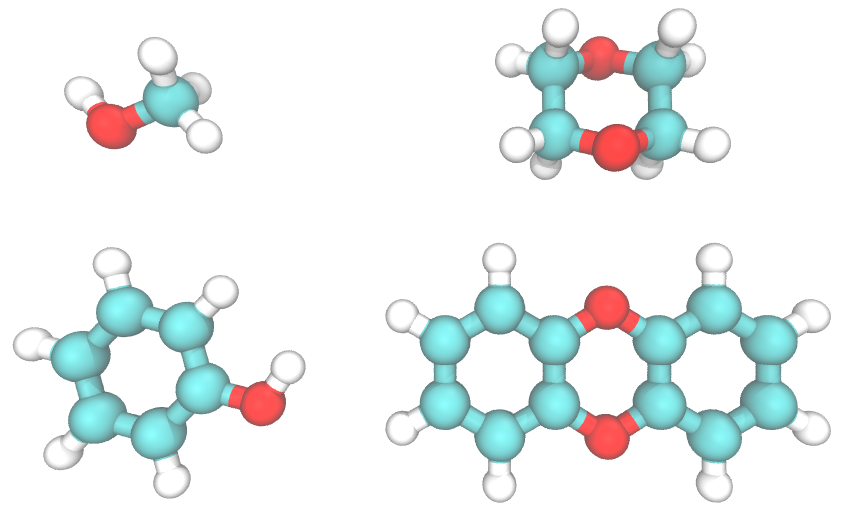
\includegraphics[width=\linewidth]{molecular_structures}
	\caption{Molecular structures.}
	\label{fig:molecular structures}
\end{figure}

For all bonded and van der Waals interactions, the solute molecules were modeled by using the General Amber Force-Field (GAFF) force field \cite{Wang_2004}.
As it is usual for this specific force field, the partial charges of the atoms was computed by using the semi-empirical AM1-BCC method \cite{Jakalian_2000, *Jakalian_2002}, which is available in the Antechamber code \cite{Wang_2006} and distributed in the Ambertools package \cite{Case_2017}.
The solvent parameter and all other simulation details are exactly as described in the previous section, including the procedure used to determine the box volume.
%In this way, the employed box side lengths and resulting densities were
%$L = 24.464~\mathrm{\AA}$ and $\rho = ~\mathrm{g/cm^3}$ for methanol,
%$L = 24.512~\mathrm{\AA}$ and $\rho = ~\mathrm{g/cm^3}$ for phenol,
%$L = 24.510~\mathrm{\AA}$ and $\rho = ~\mathrm{g/cm^3}$ for 1,4-dioxane, and
%$L = 24.560~\mathrm{\AA}$ and $\rho = ~\mathrm{g/cm^3}$ for dibenzo-p-dioxin.
In this way, the employed box side lengths were $24.464~\mathrm{\AA}$ for methanol, $24.512~\mathrm{\AA}$ for phenol, $24.510~\mathrm{\AA}$ for 1,4-dioxane, and $24.560~\mathrm{\AA}$ for dibenzo-p-dioxin.

Once again, the total simulation time was $4.5~\mathrm{ns}$, out of which $3.6~\mathrm{ns}$ was taken as production time.
To compute the van der Waals contribution to the solvation free energy, we employed the same 21 states of $\lambda_\mathrm{vdW}$.
Fewer states are required for computing the electrostatic contribution, which could be done by defining 11 equally spaced states of $\lambda_\mathrm{coul}$ from $0$ to $1$.

\begin{figure}
	\centering
	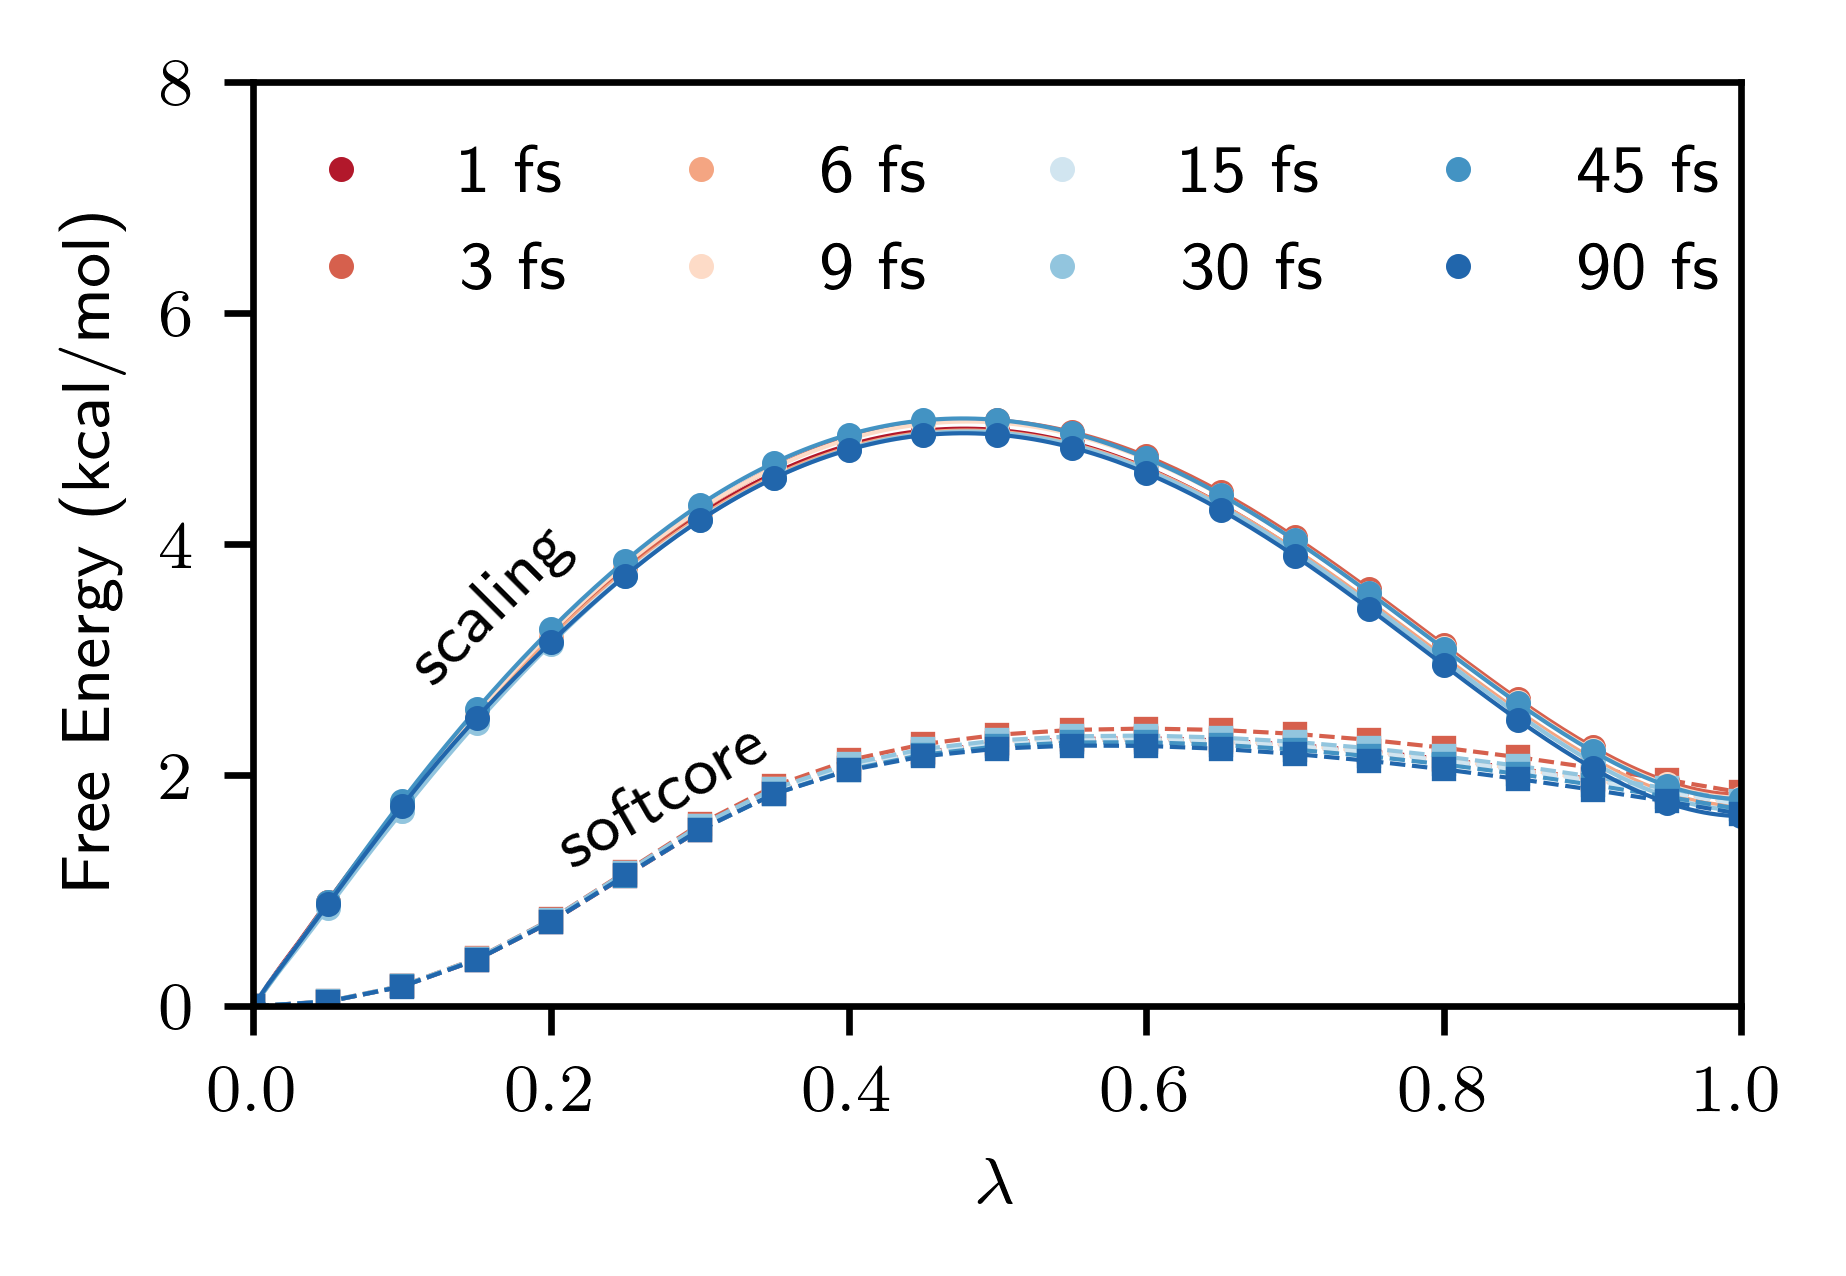
\includegraphics{gaff_methanol_vdw_free_energy_profiles}
	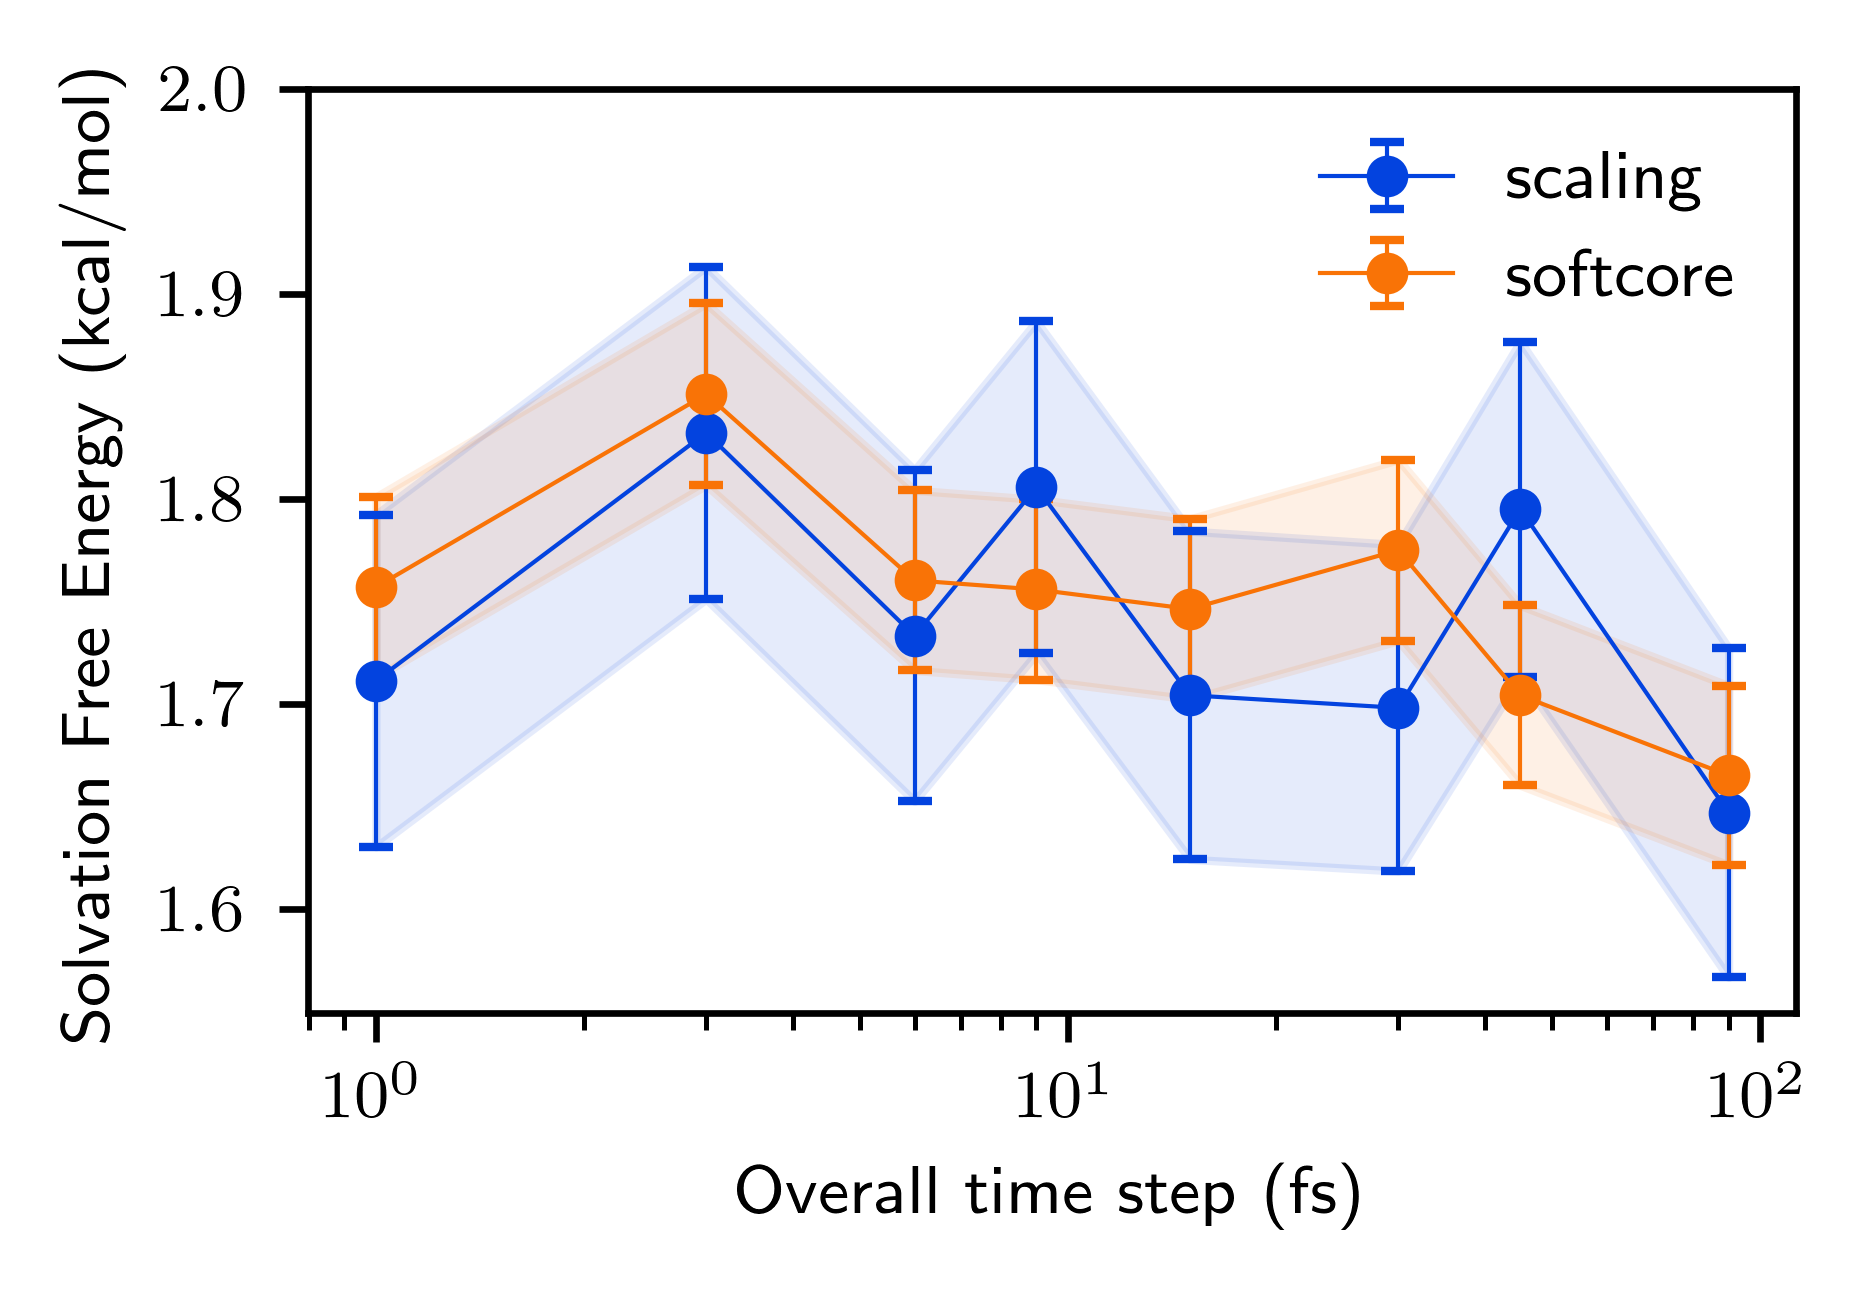
\includegraphics{gaff_methanol_vdw_free_energies}
	\caption{GAFF methanol Free Energy.}
	\label{fig:methanol vdw free energy}
\end{figure}

\begin{figure}
	\centering
	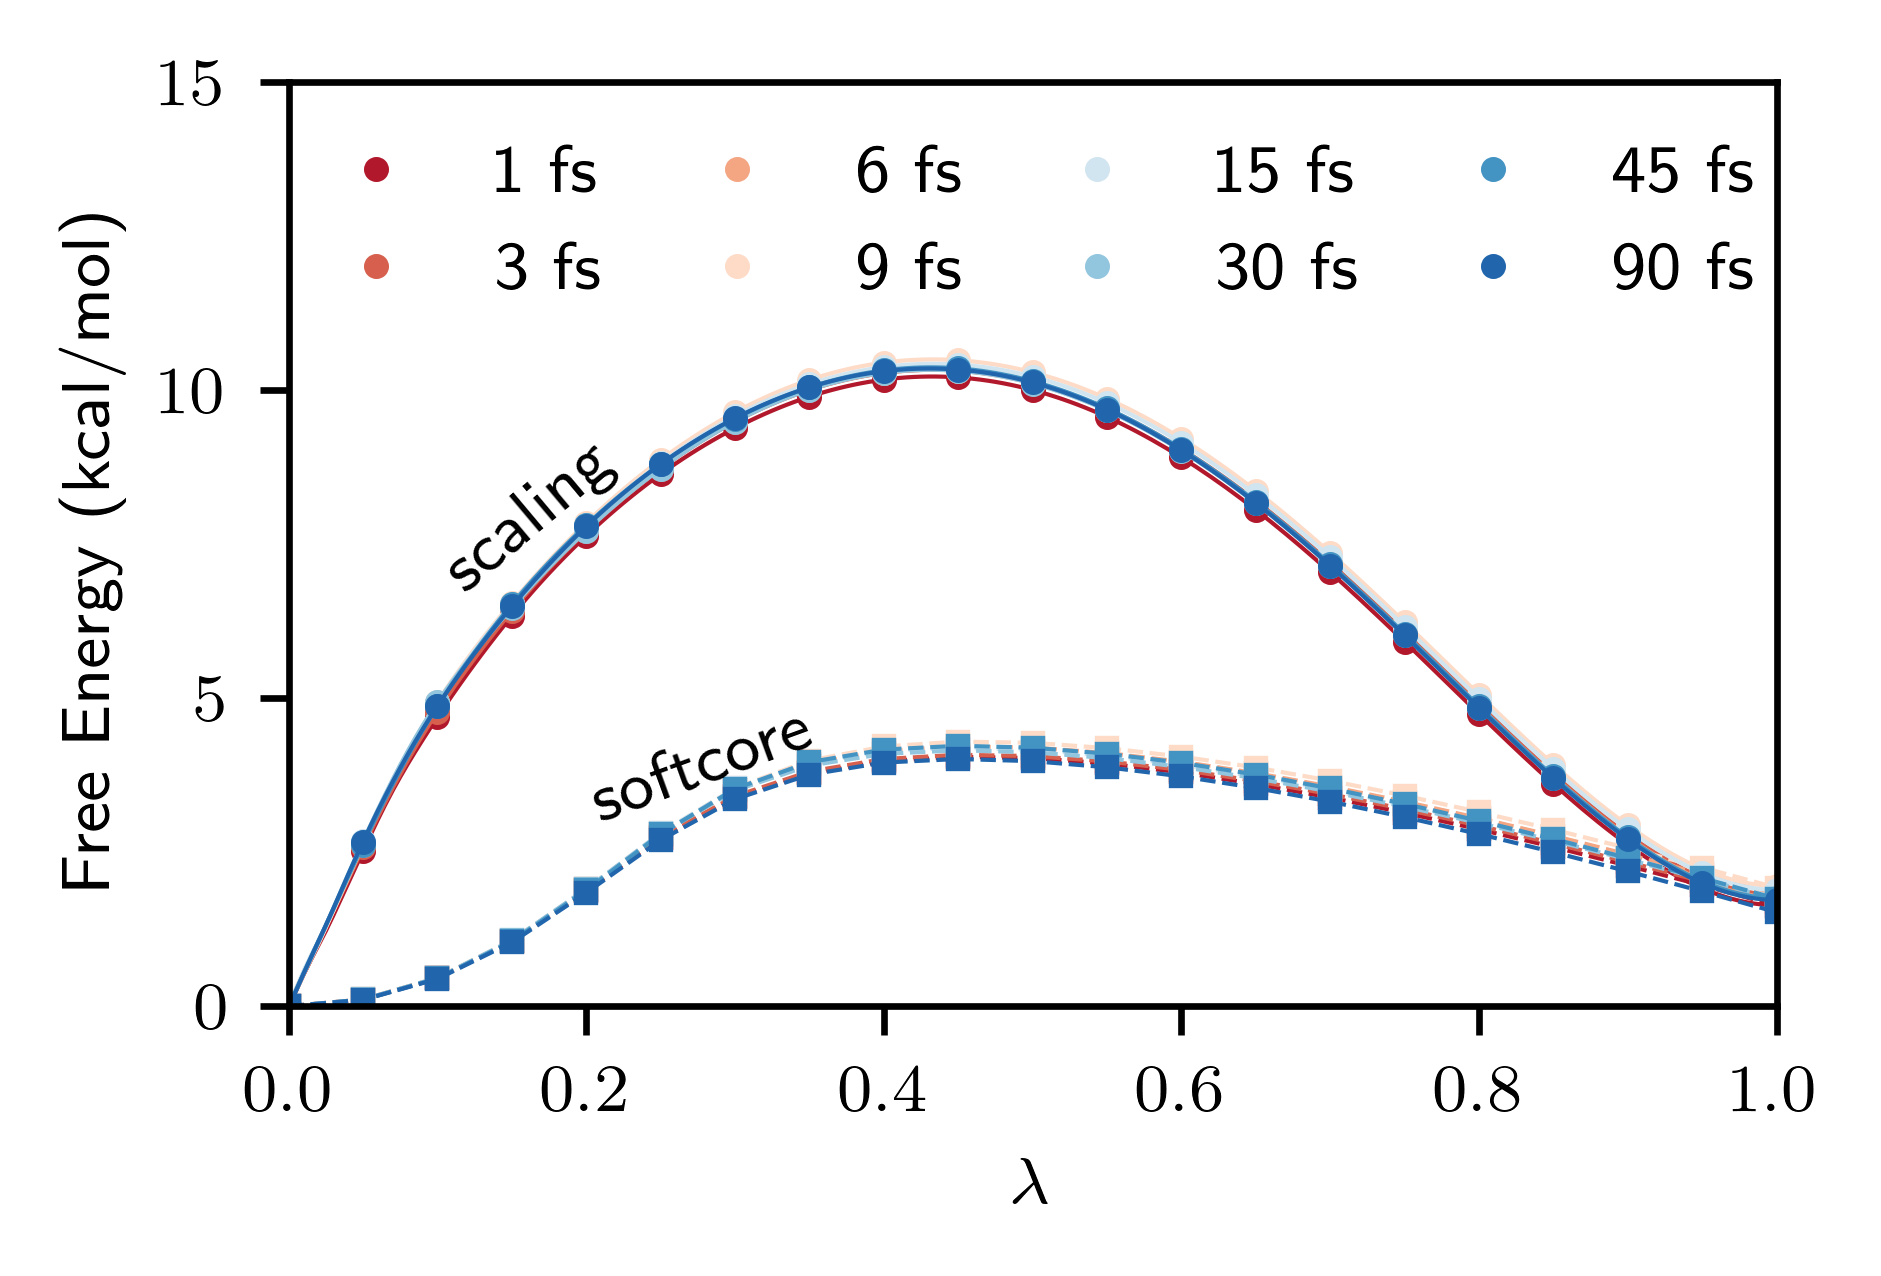
\includegraphics{gaff_phenol_vdw_free_energy_profiles}
	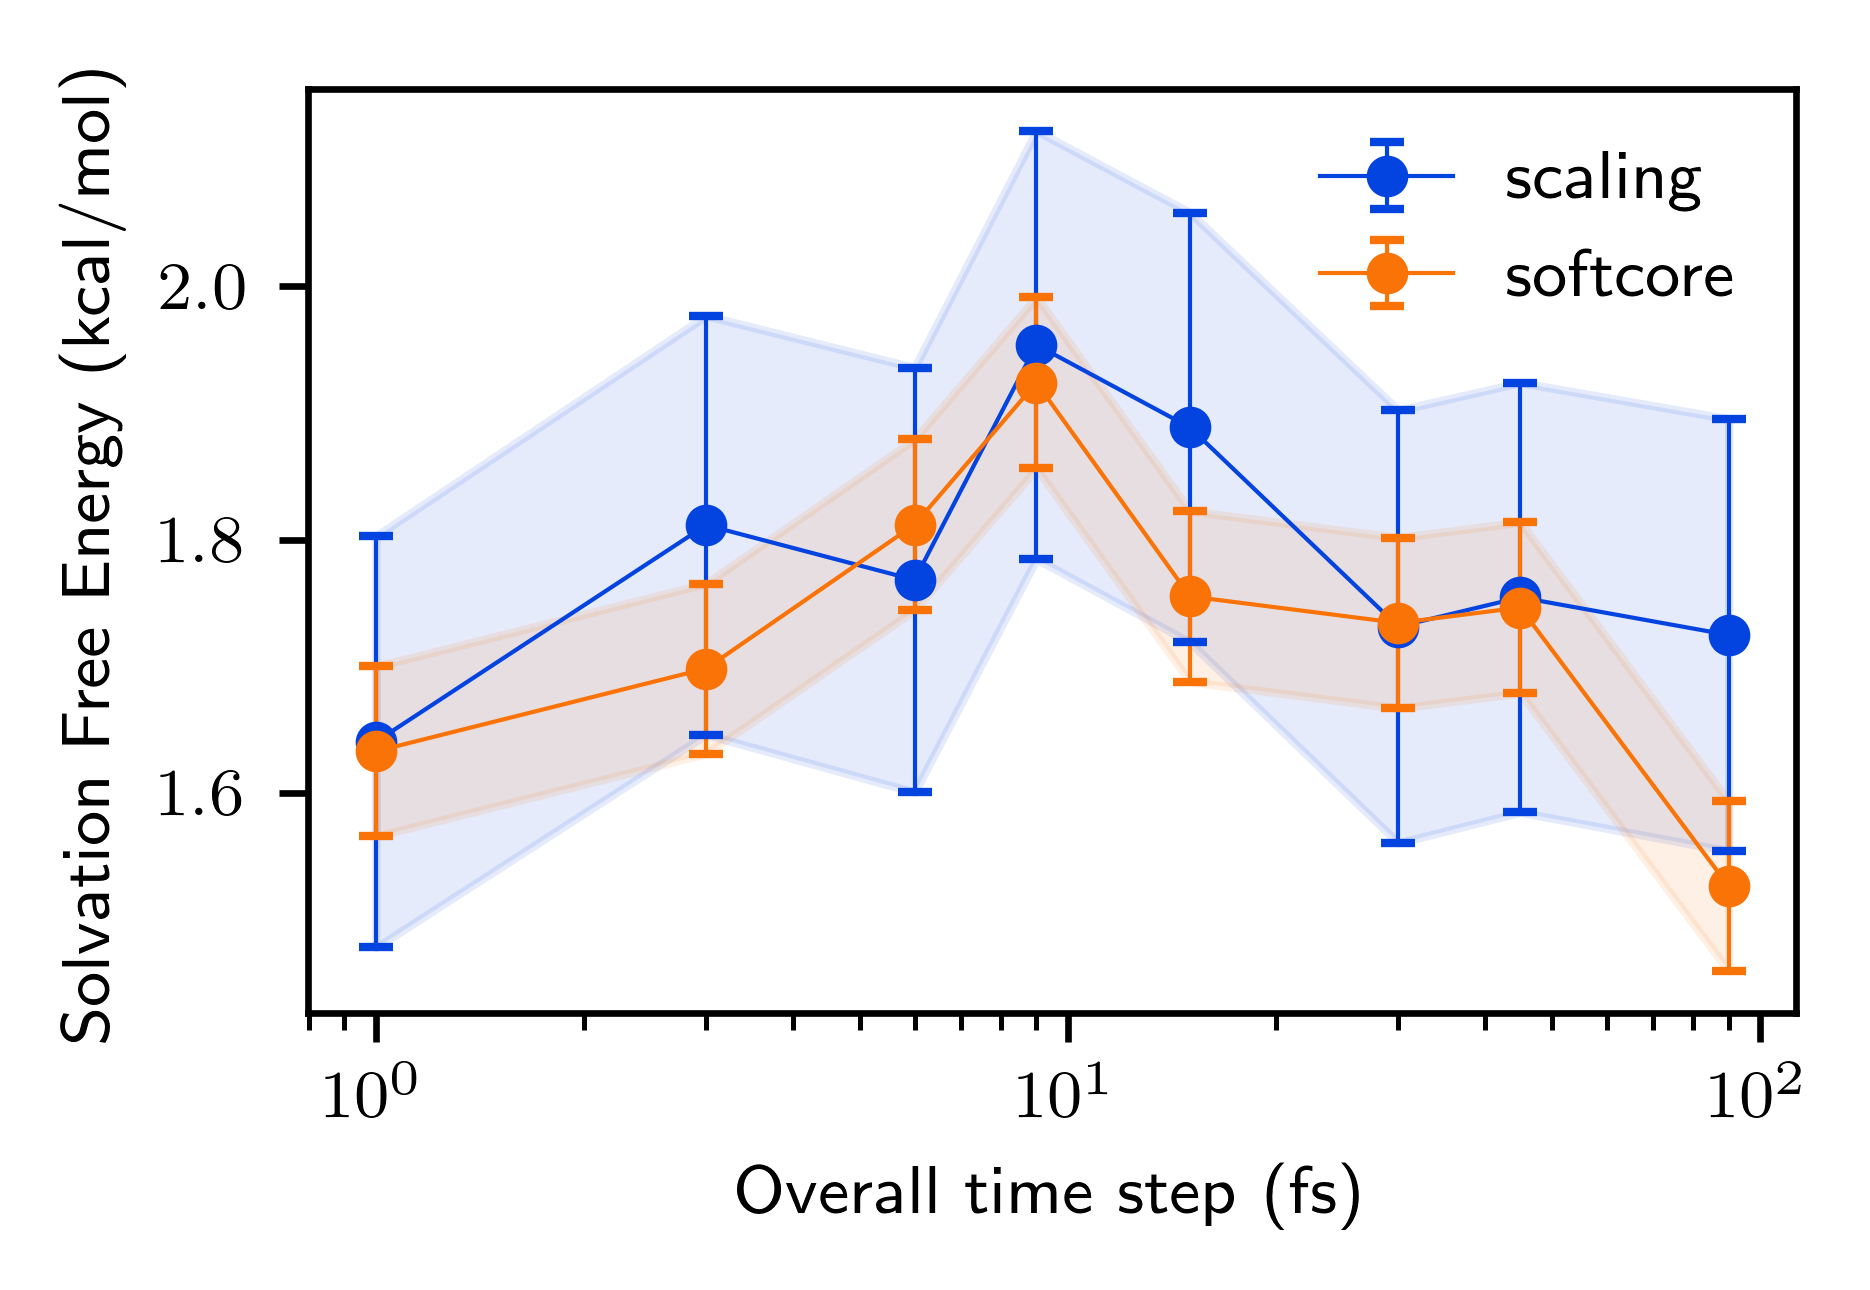
\includegraphics{gaff_phenol_vdw_free_energies}
	\caption{GAFF Phenol Free Energy.}
	\label{fig:phenol vdw free energy}
\end{figure}

\begin{figure}
	\centering
	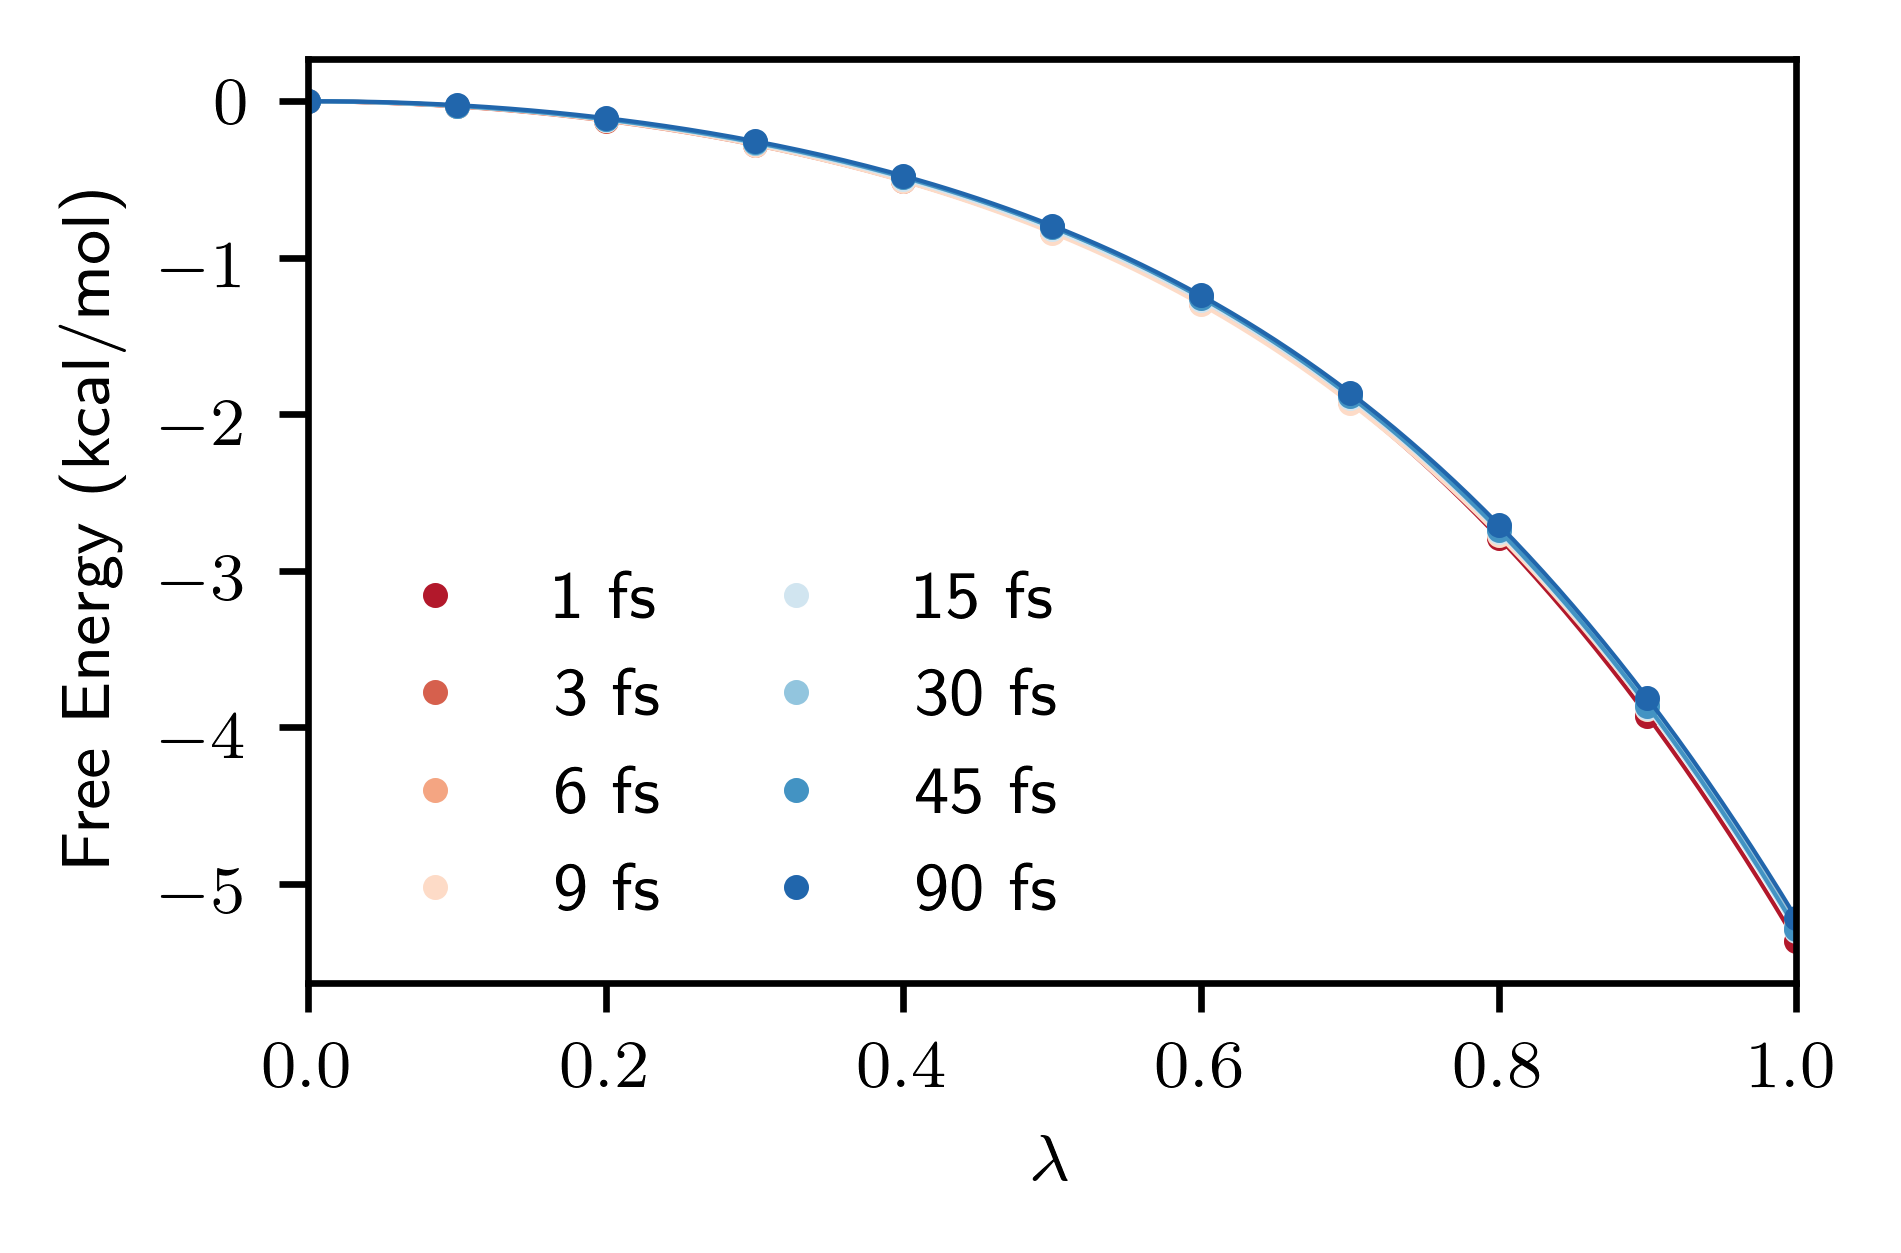
\includegraphics{gaff_methanol_coul_free_energy_profiles}
	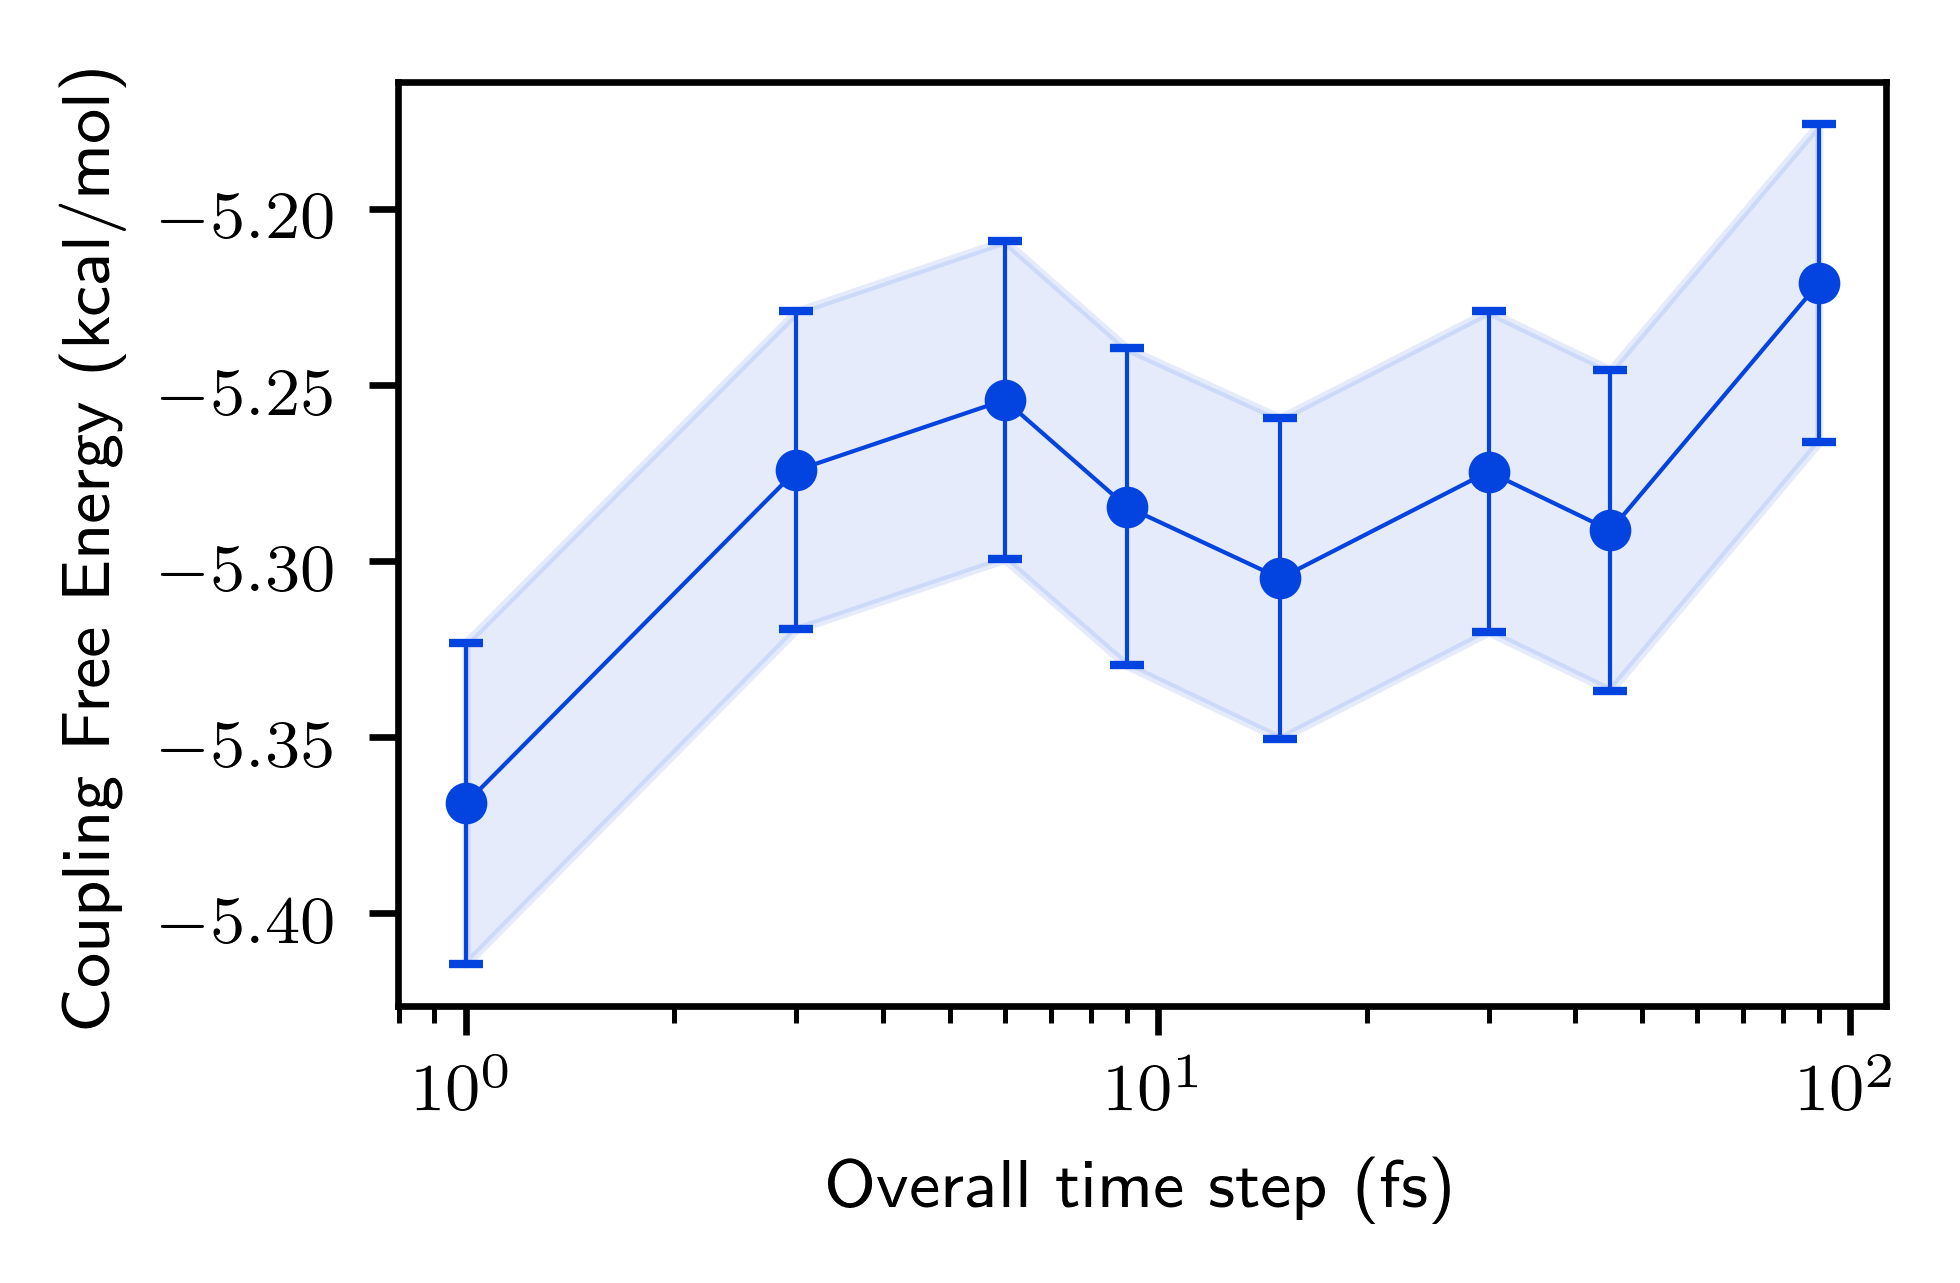
\includegraphics{gaff_methanol_coul_free_energies}
	\caption{GAFF methanol Free Energy.}
	\label{fig:methanol coulomb free energy}
\end{figure}


\begin{figure}
	\centering
	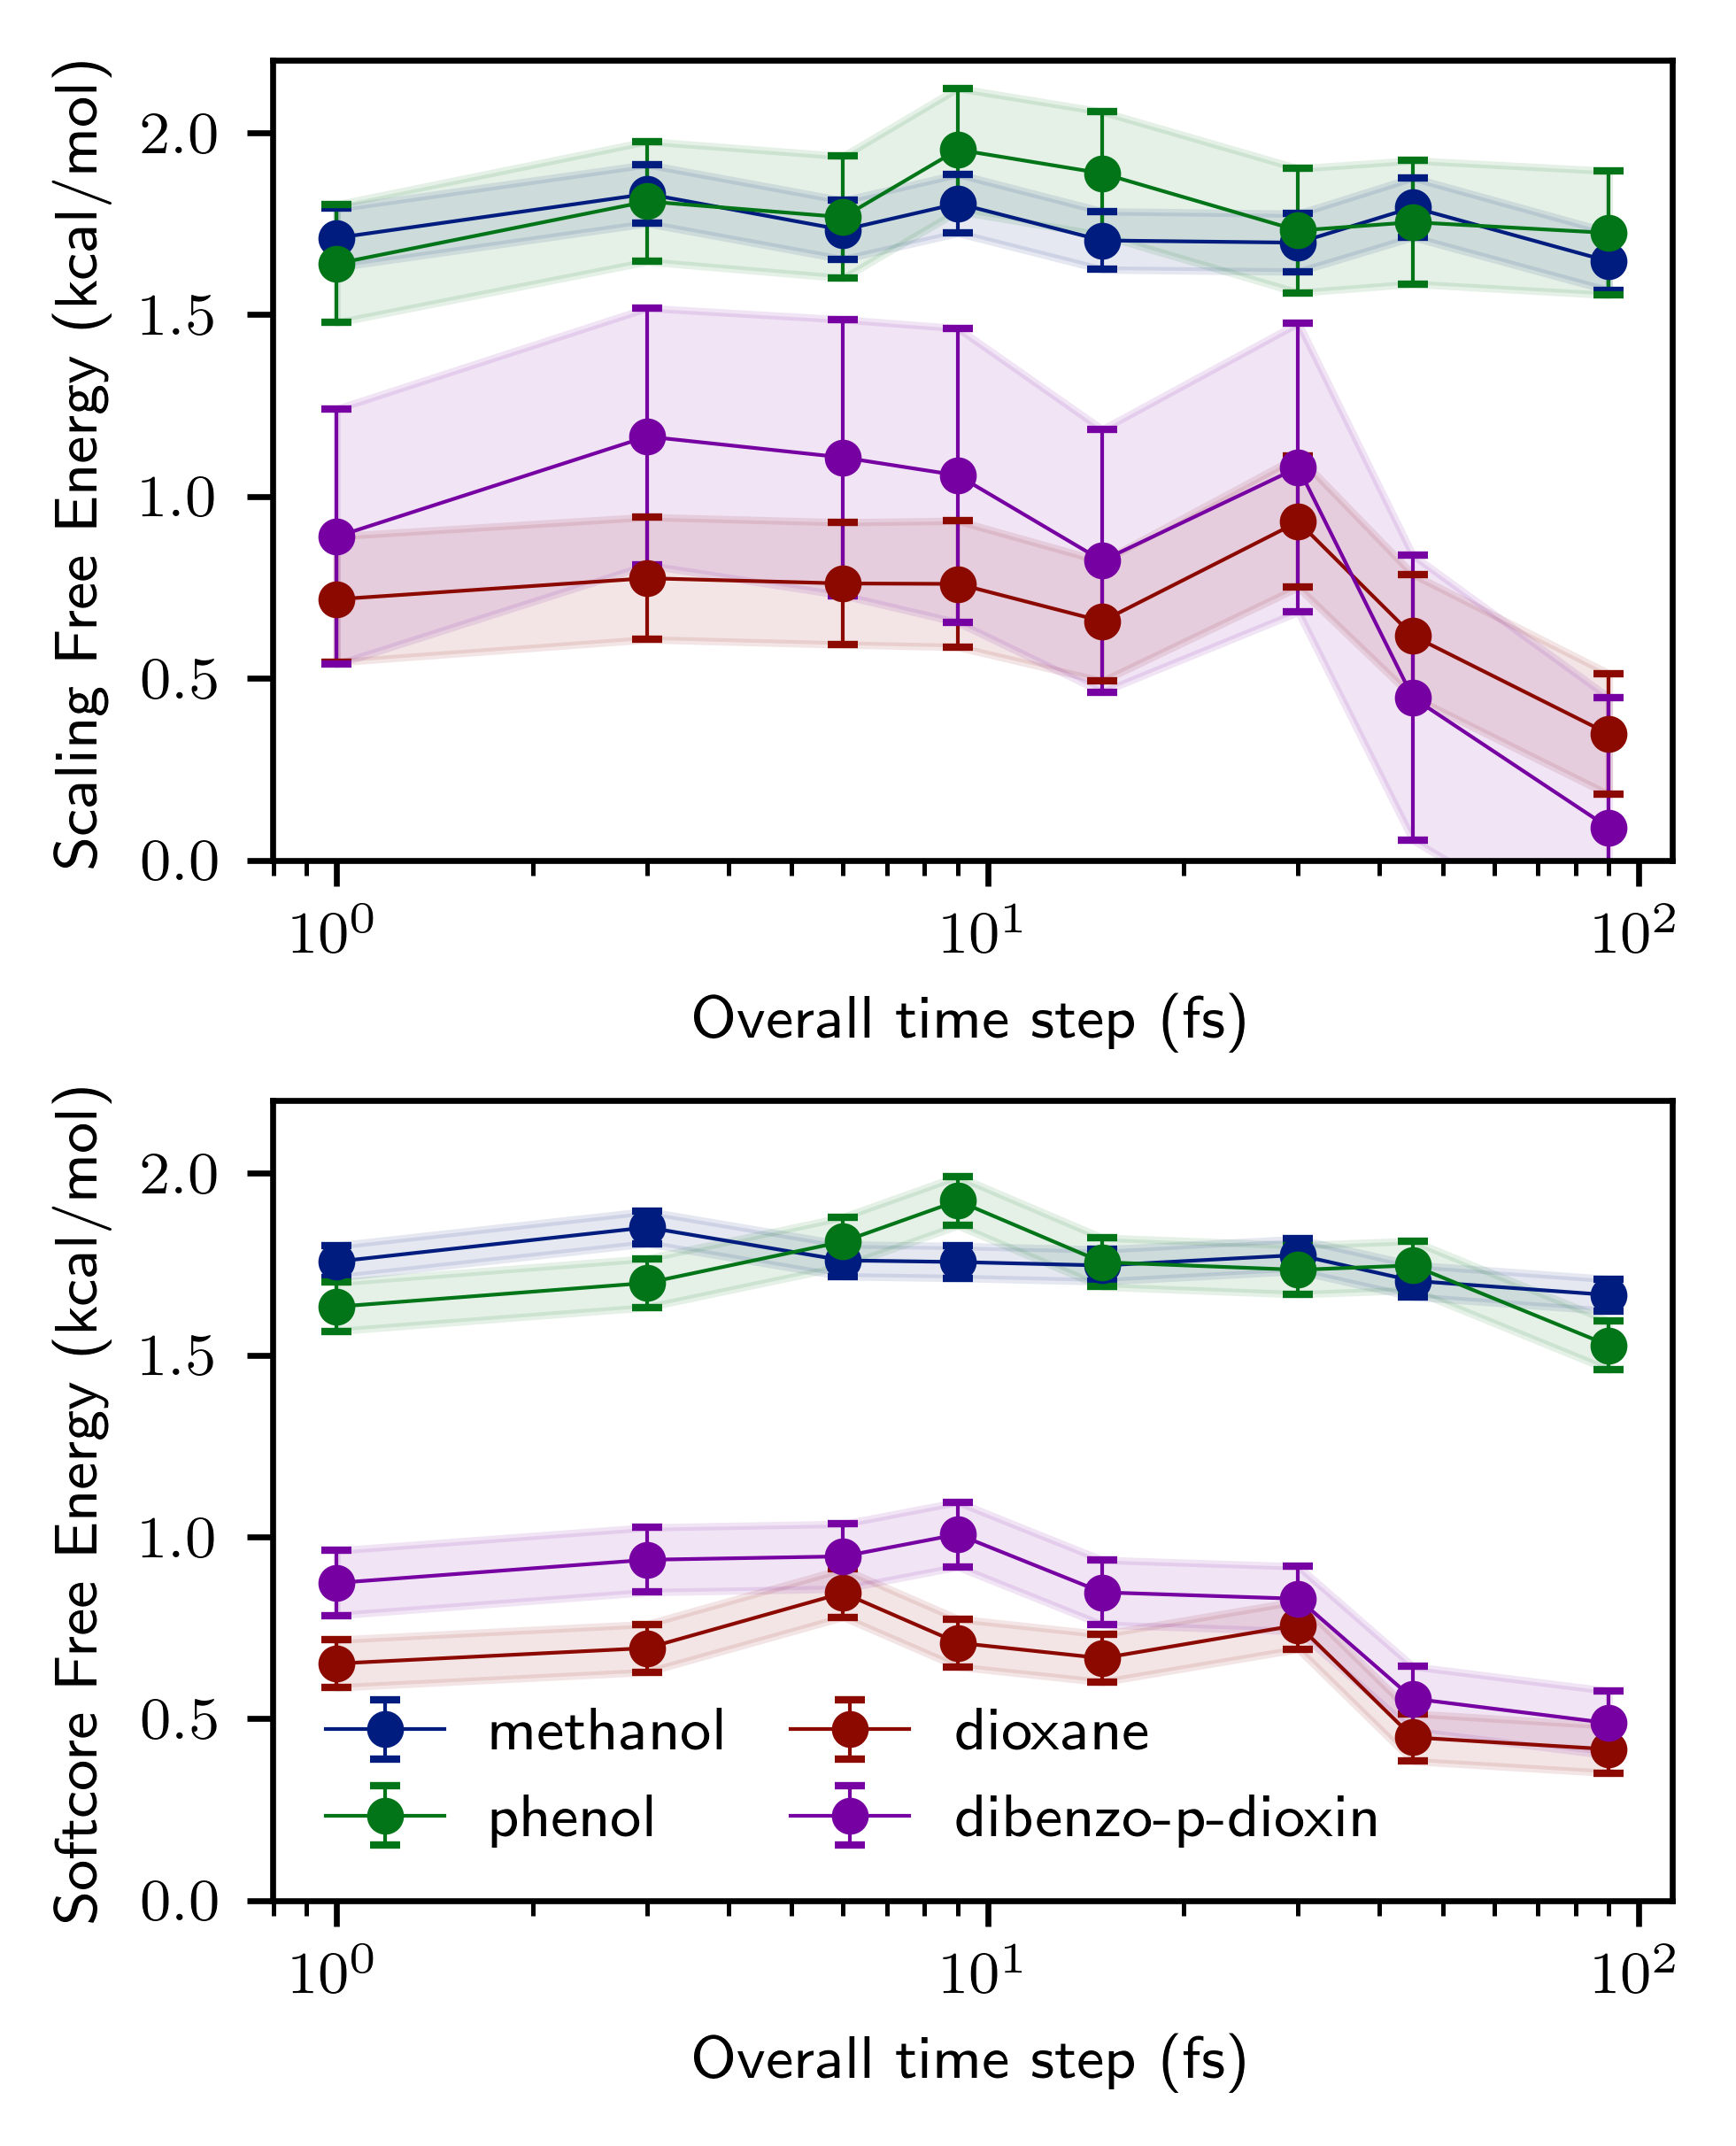
\includegraphics{all_molecules_vdw_free_energies}
	\caption{van der Waals free energies}
	\label{fig:van der Waals free energies of all molecules}
\end{figure}

\begin{figure}
	\centering
	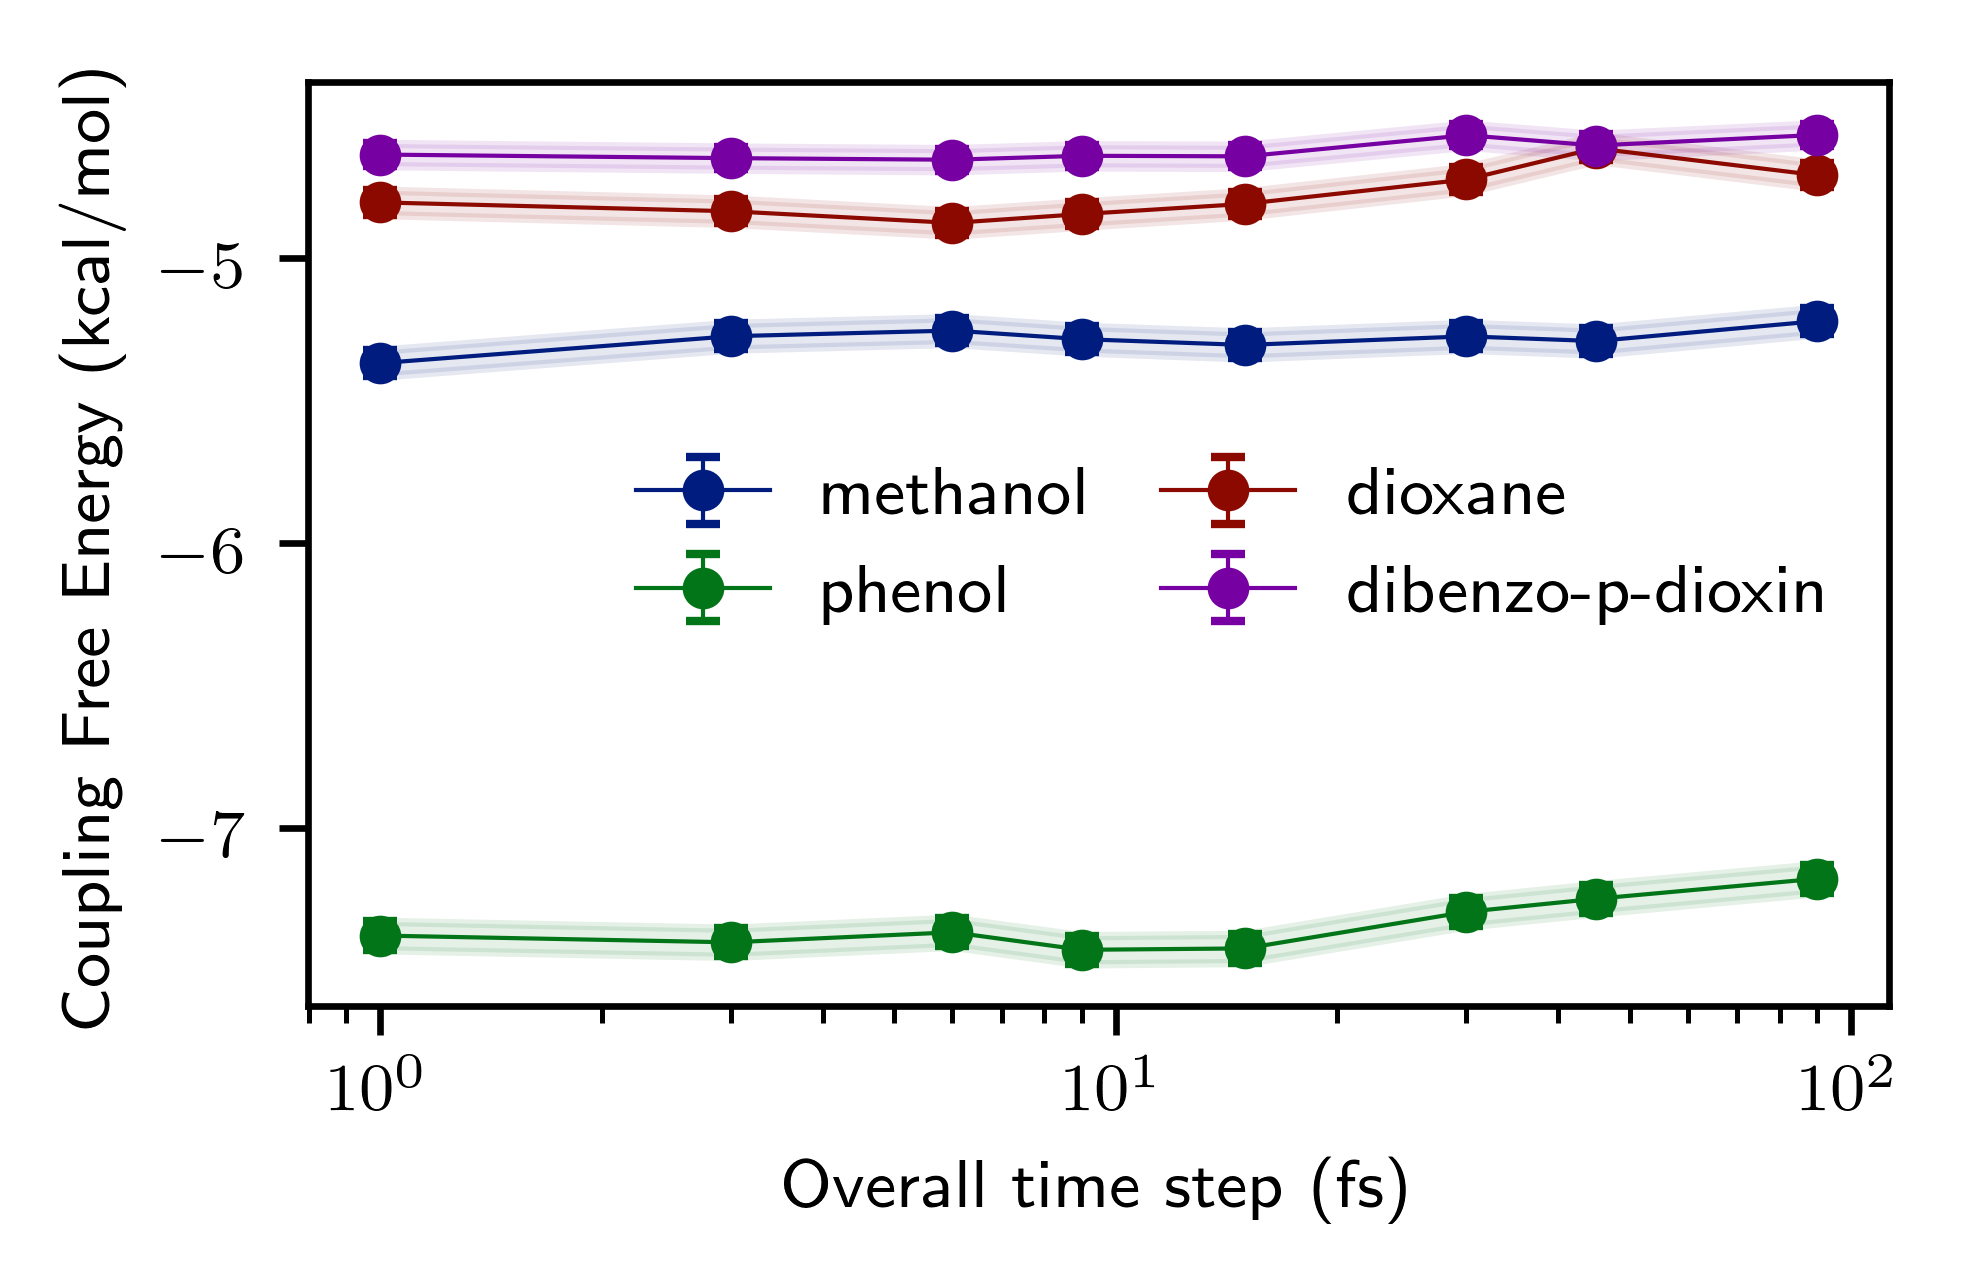
\includegraphics{all_molecules_coul_free_energies}
	\caption{Coulomb free energies}
	\label{fig:Coulomb free energies of all molecules}
\end{figure}

\begin{figure}
	\centering
	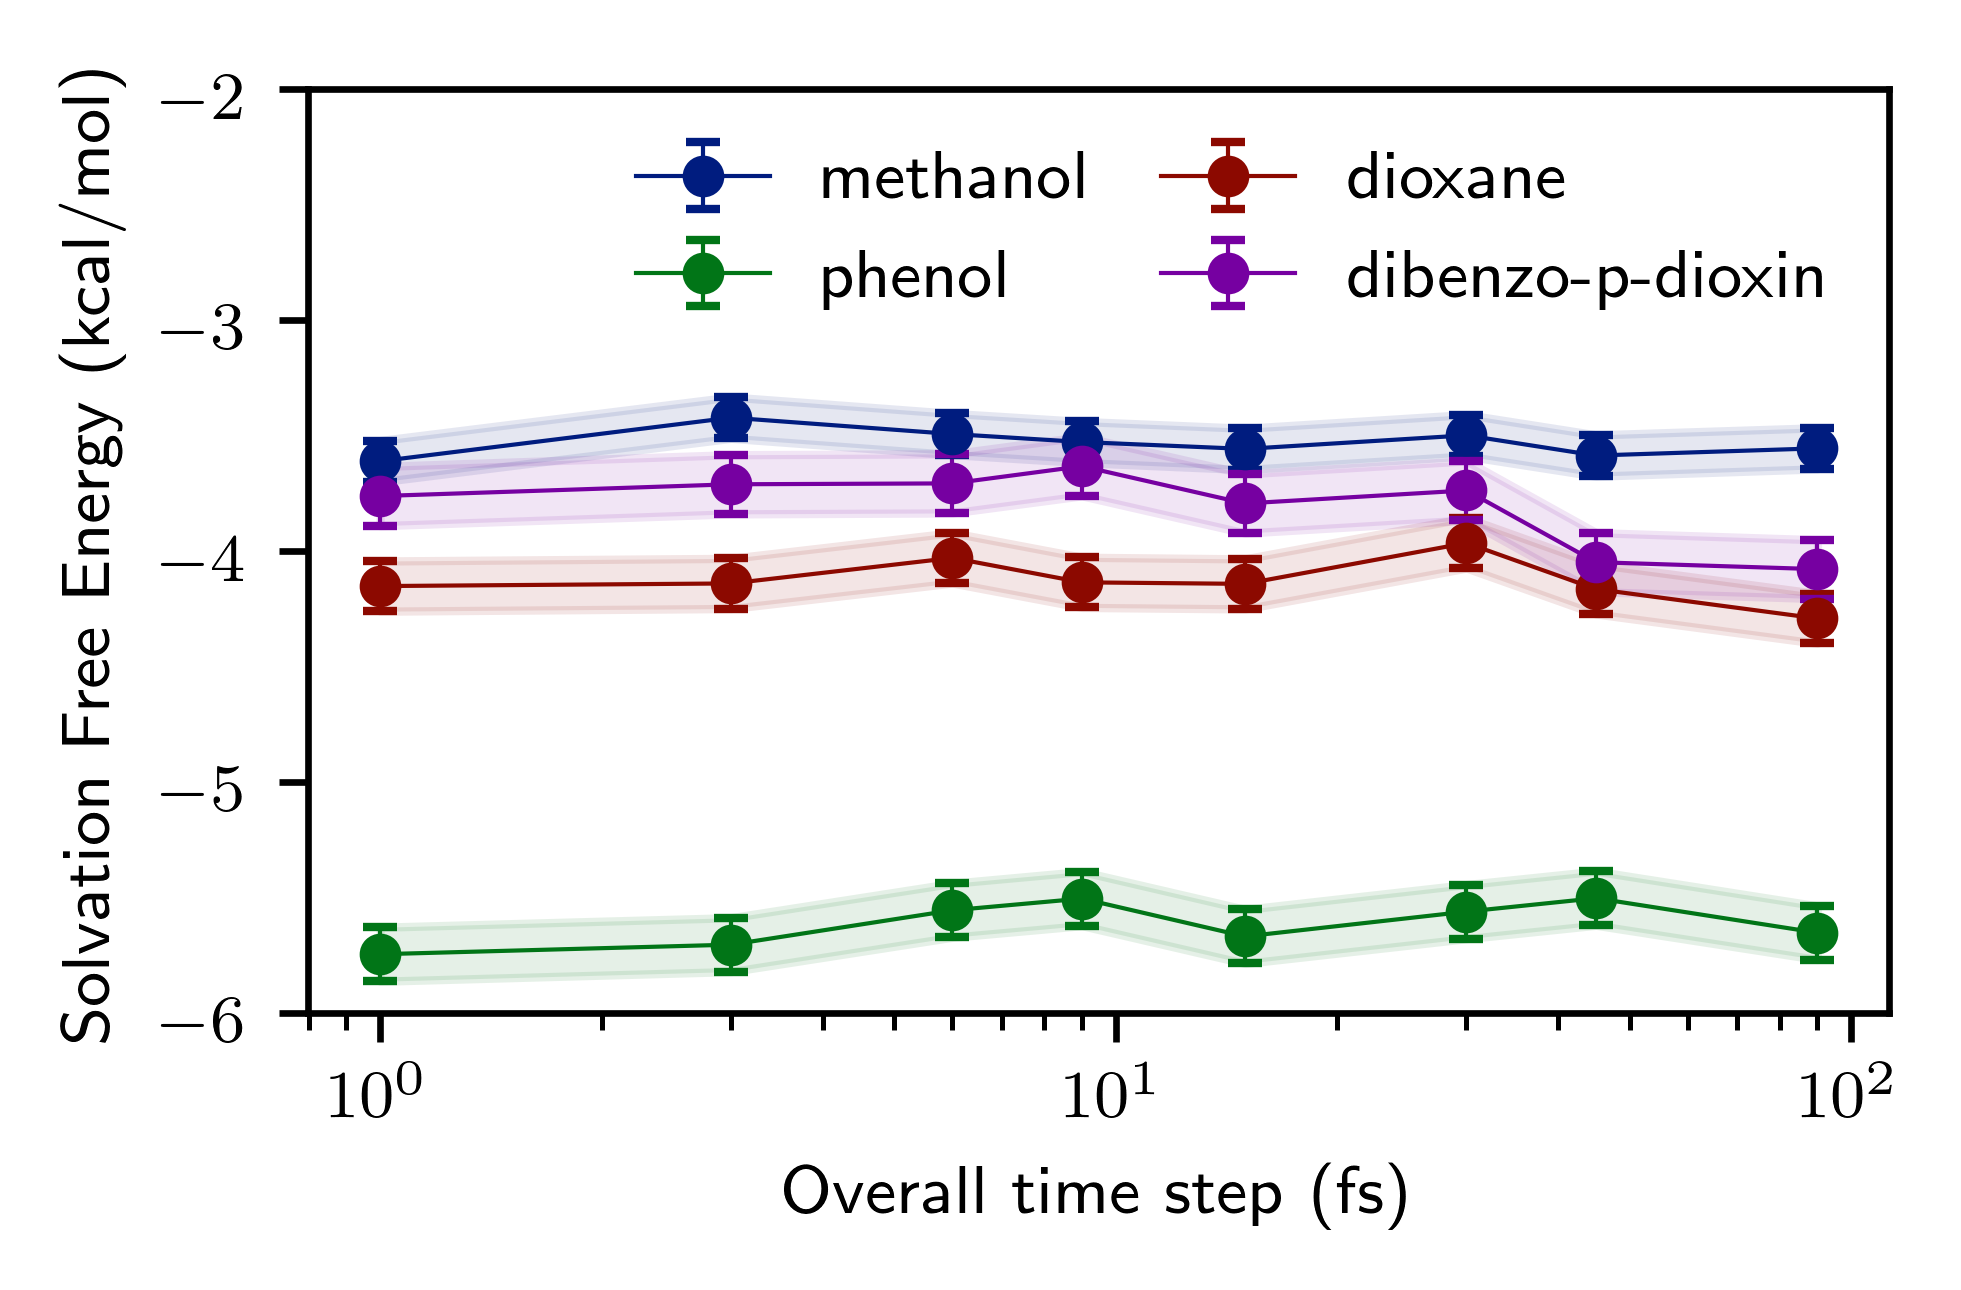
\includegraphics{all_molecules_total_free_energies}
	\caption{Total free energies}
	\label{fig:Total free energies of all molecules}
\end{figure}


\begin{table*}
	\begin{ruledtabular}
		\begin{tabular}{lcccccc}
			{}                & Exp. & FreeSolv \cite{Mobley_2014_2, Duarte_ramos_matos_2017} & $\Delta t = 1~\mathrm{fs}$  & $\Delta t = 6~\mathrm{fs}$  & $\Delta t = 30~\mathrm{fs}$ & $\Delta t = 90~\mathrm{fs}$ \\
			\hline
            methane & $+2.0 \pm 0.2$ \cite{Abraham_1990} & $+2.45 \pm 0.01$ & $+2.17 \pm 0.02$ & $+2.26 \pm 0.02$ & $+2.20 \pm 0.02$ & $+2.05 \pm 0.02$ \\
			methanol          & $-5.1 \pm 0.6$ \cite{Rizzo_2006}  & $-3.49 \pm 0.02$ & $-3.61 \pm 0.09$ & $-3.49 \pm 0.09$ & $-3.50 \pm 0.09$ & $-3.56 \pm 0.09$ \\
			phenol            & $-6.6 \pm 0.2$ \cite{Abraham_1990} & $-5.71 \pm 0.03$ & $-5.75 \pm 0.12$ & $-5.56 \pm 0.12$ & $-5.56 \pm 0.12$ & $-5.65 \pm 0.12$ \\
			1,4-dioxane       & $-5.06 \pm 0.6$ \cite{Rizzo_2006} & $-4.27 \pm 0.02$ & $-4.15 \pm 0.11$ & $-4.03 \pm 0.11$ & $-3.97 \pm 0.11$ & $-4.29 \pm 0.11$ \\
			dibenzo-p-dioxin  & $-3.15 \pm 0.1$ \cite{Geballe_2012} & $-4.9 \pm 0.02$ & $-3.76 \pm 0.13$ & $-3.71 \pm 0.13$ & $-3.74 \pm 0.13$ & $-4.08 \pm 0.13$ \\
		\end{tabular}
	\end{ruledtabular}
\end{table*}

\appendix

\begin{figure}
	\centering
	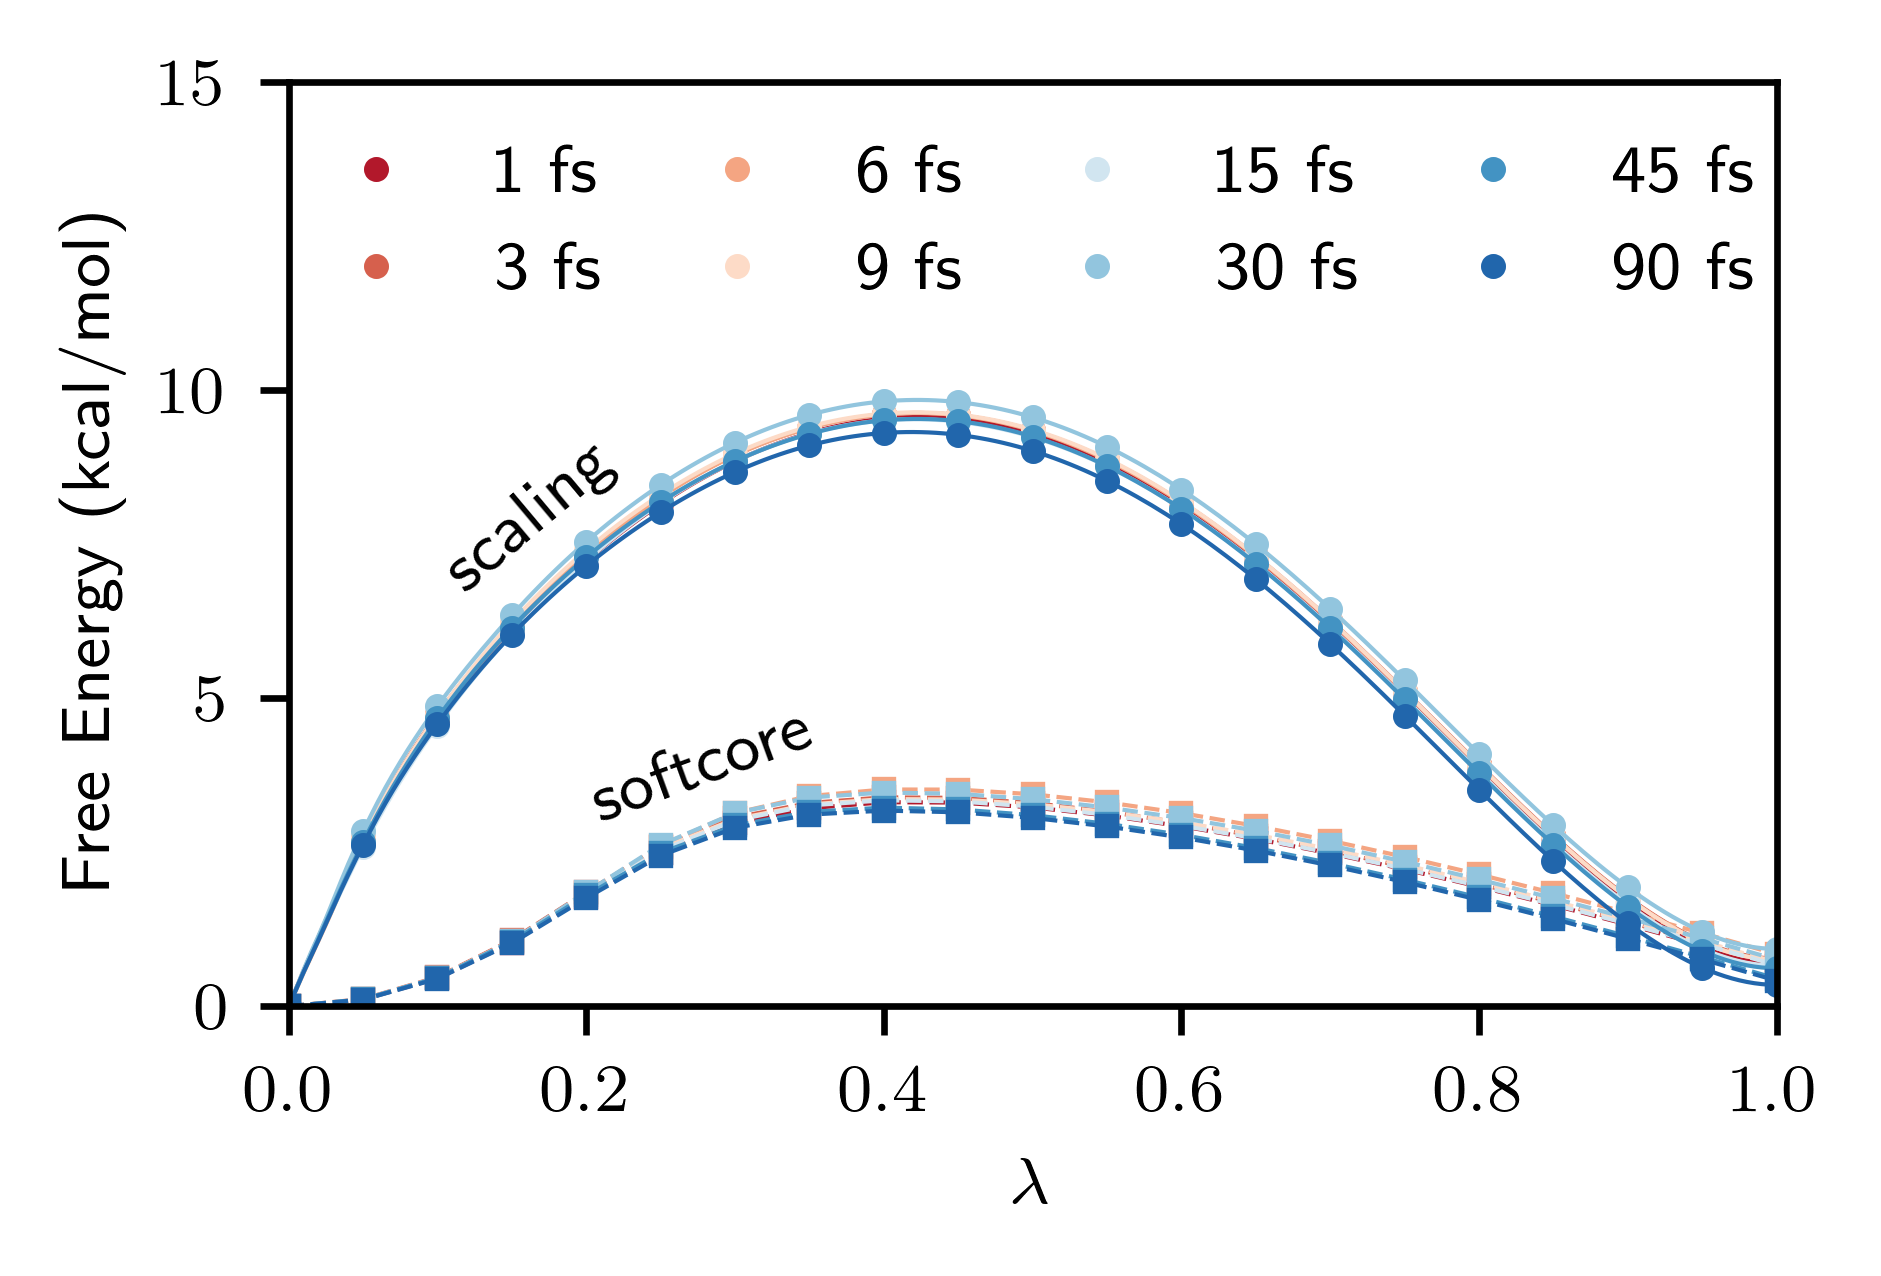
\includegraphics{gaff_dioxane_vdw_free_energy_profiles}
	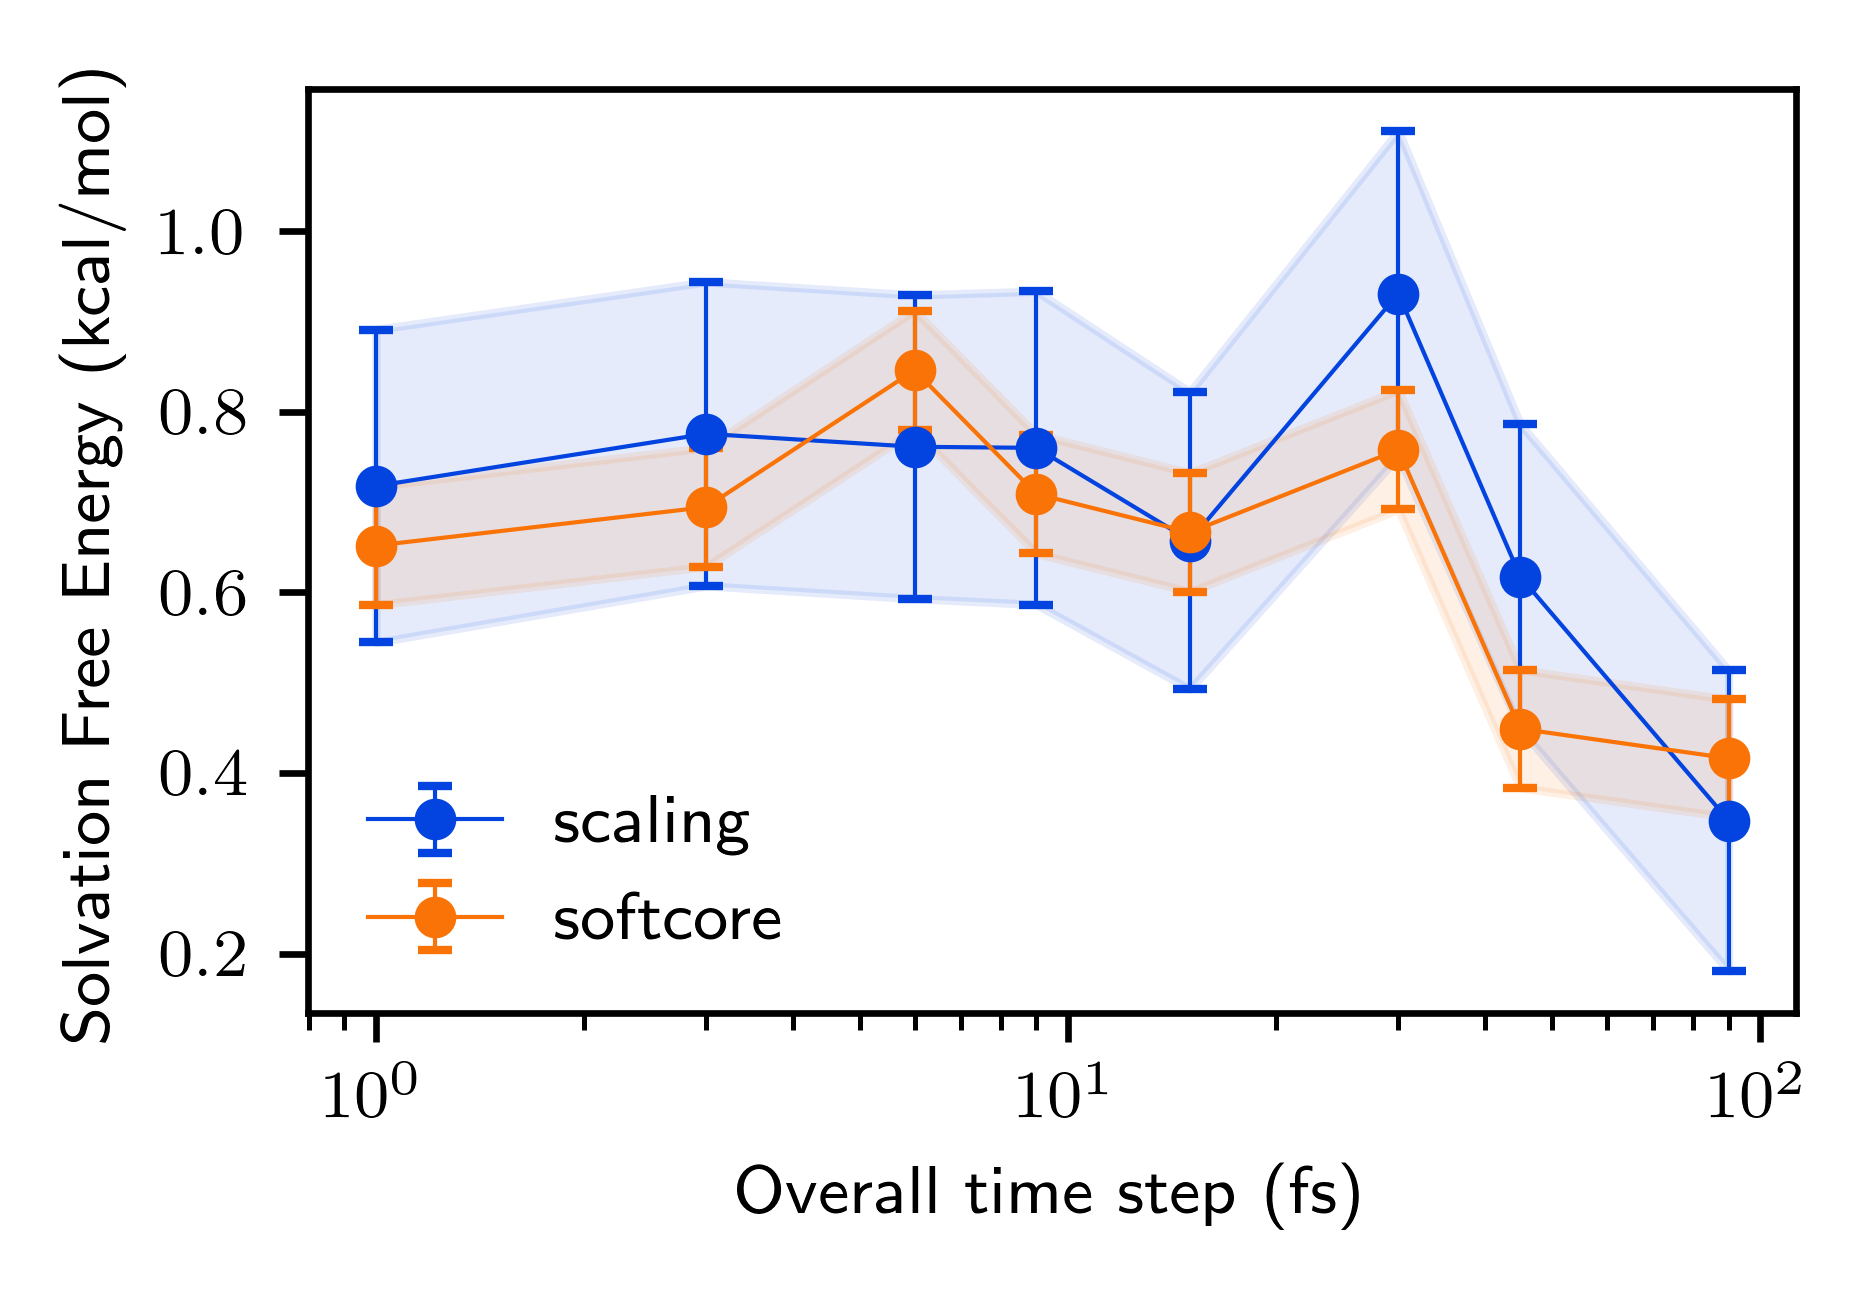
\includegraphics{gaff_dioxane_vdw_free_energies}
	\caption{GAFF 1,4-dioxane Free Energy.}
	\label{fig:dioxane vdw free energy}
\end{figure}

\begin{figure}
	\centering
	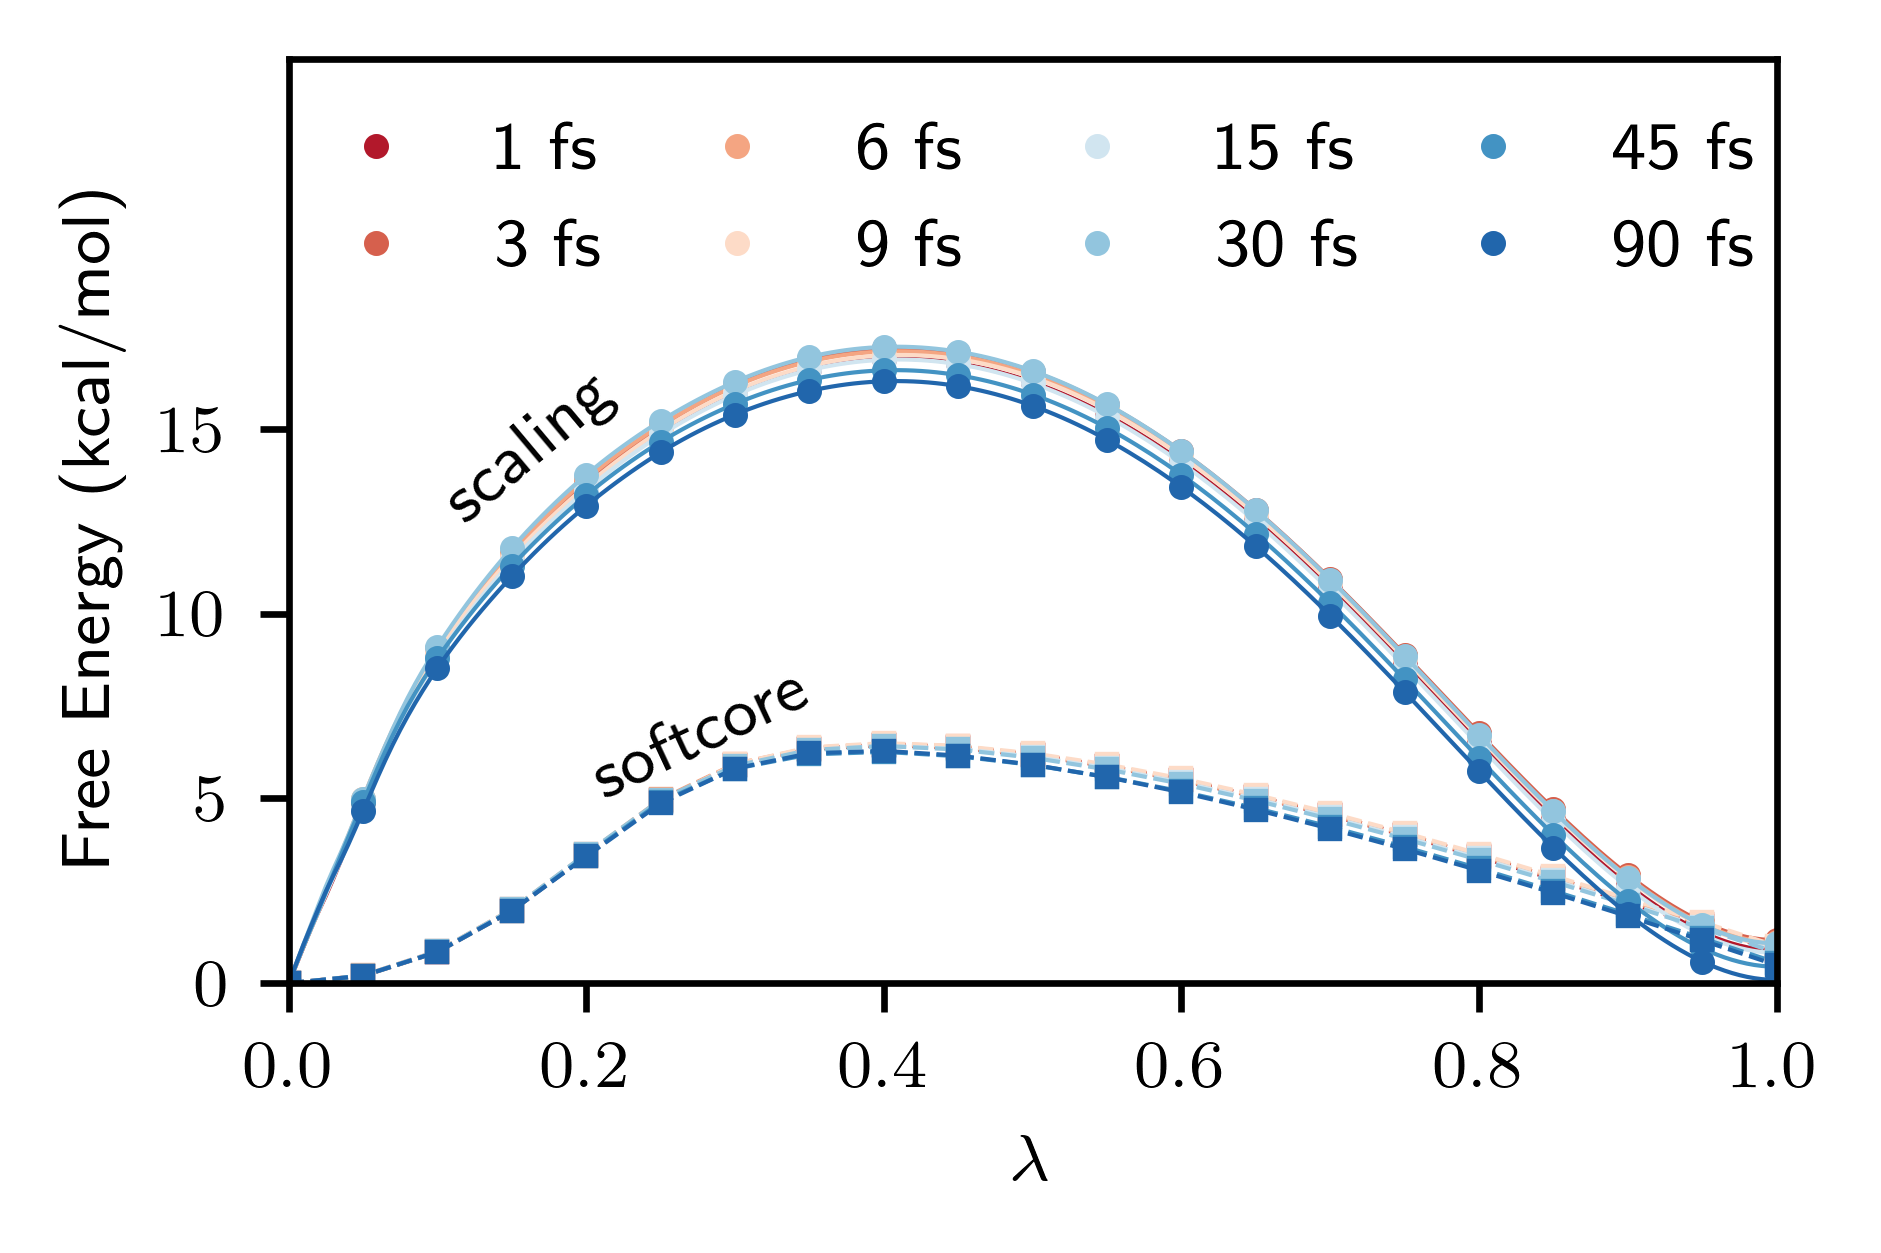
\includegraphics{gaff_dibenzo-p-dioxin_vdw_free_energy_profiles}
	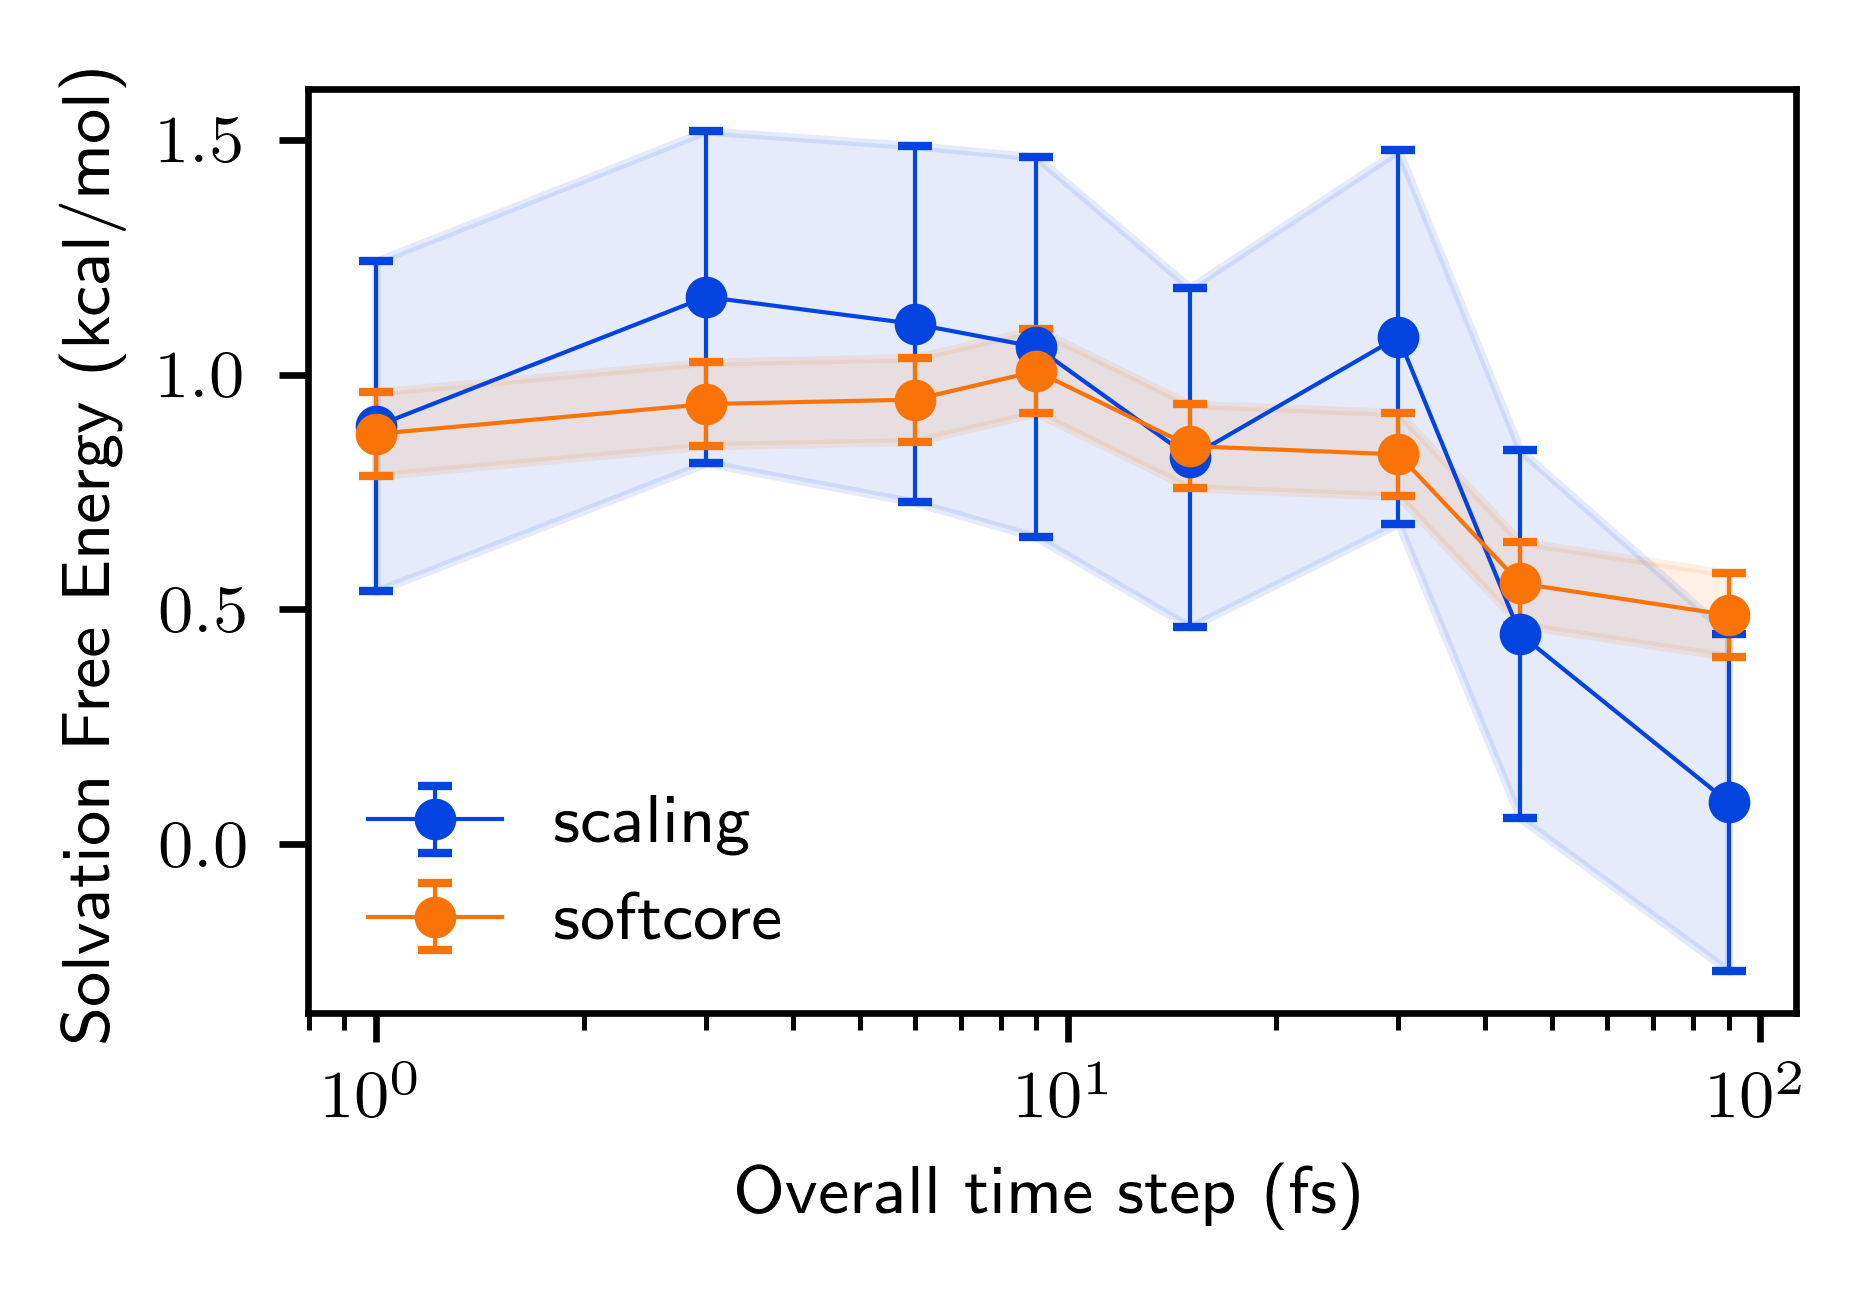
\includegraphics{gaff_dibenzo-p-dioxin_vdw_free_energies}
	\caption{GAFF dibenzo-p-dioxin Free Energy.}
	\label{fig:dibenzo-p-dioxin vdw free energy}
\end{figure}

\begin{figure}
	\centering
	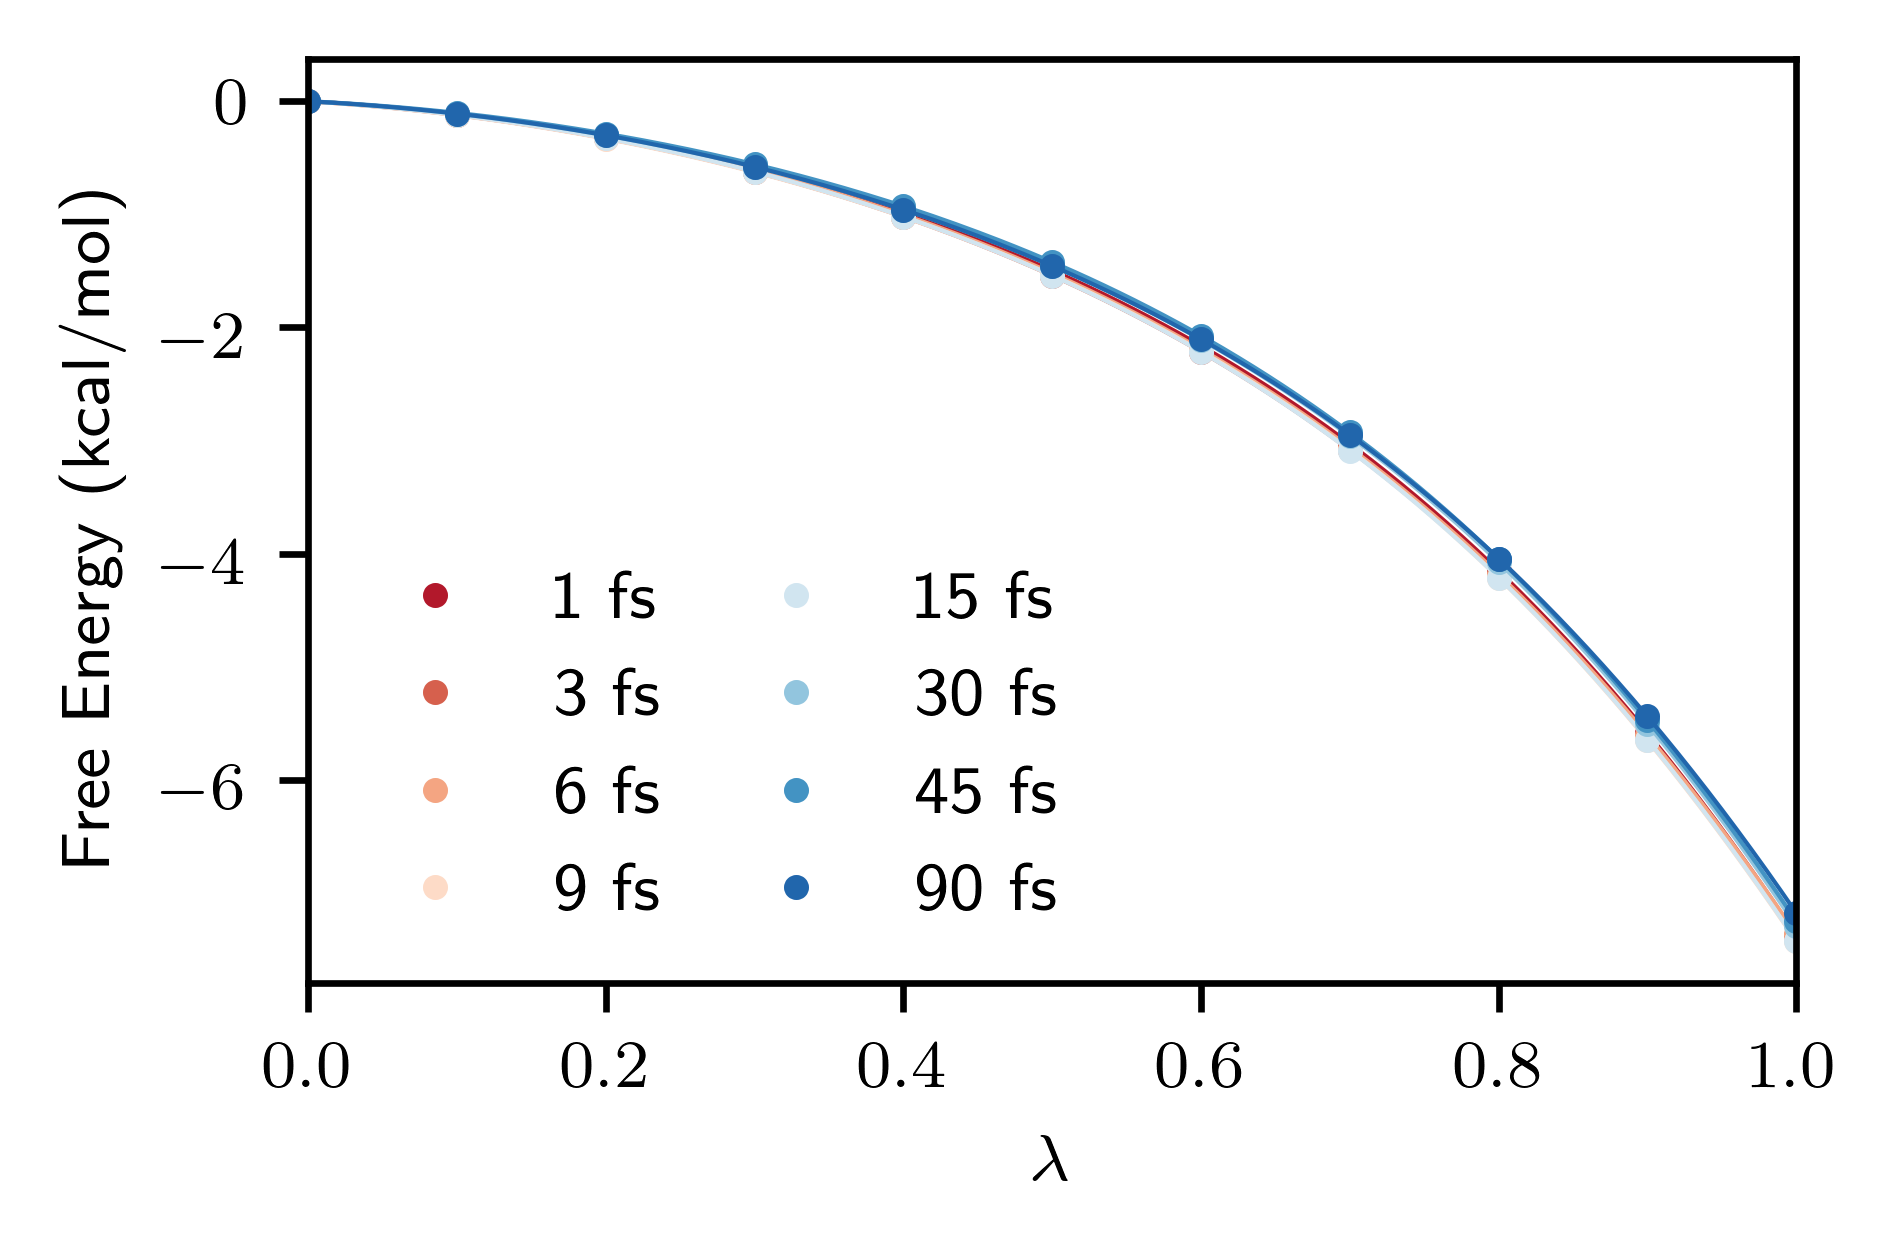
\includegraphics{gaff_phenol_coul_free_energy_profiles}
	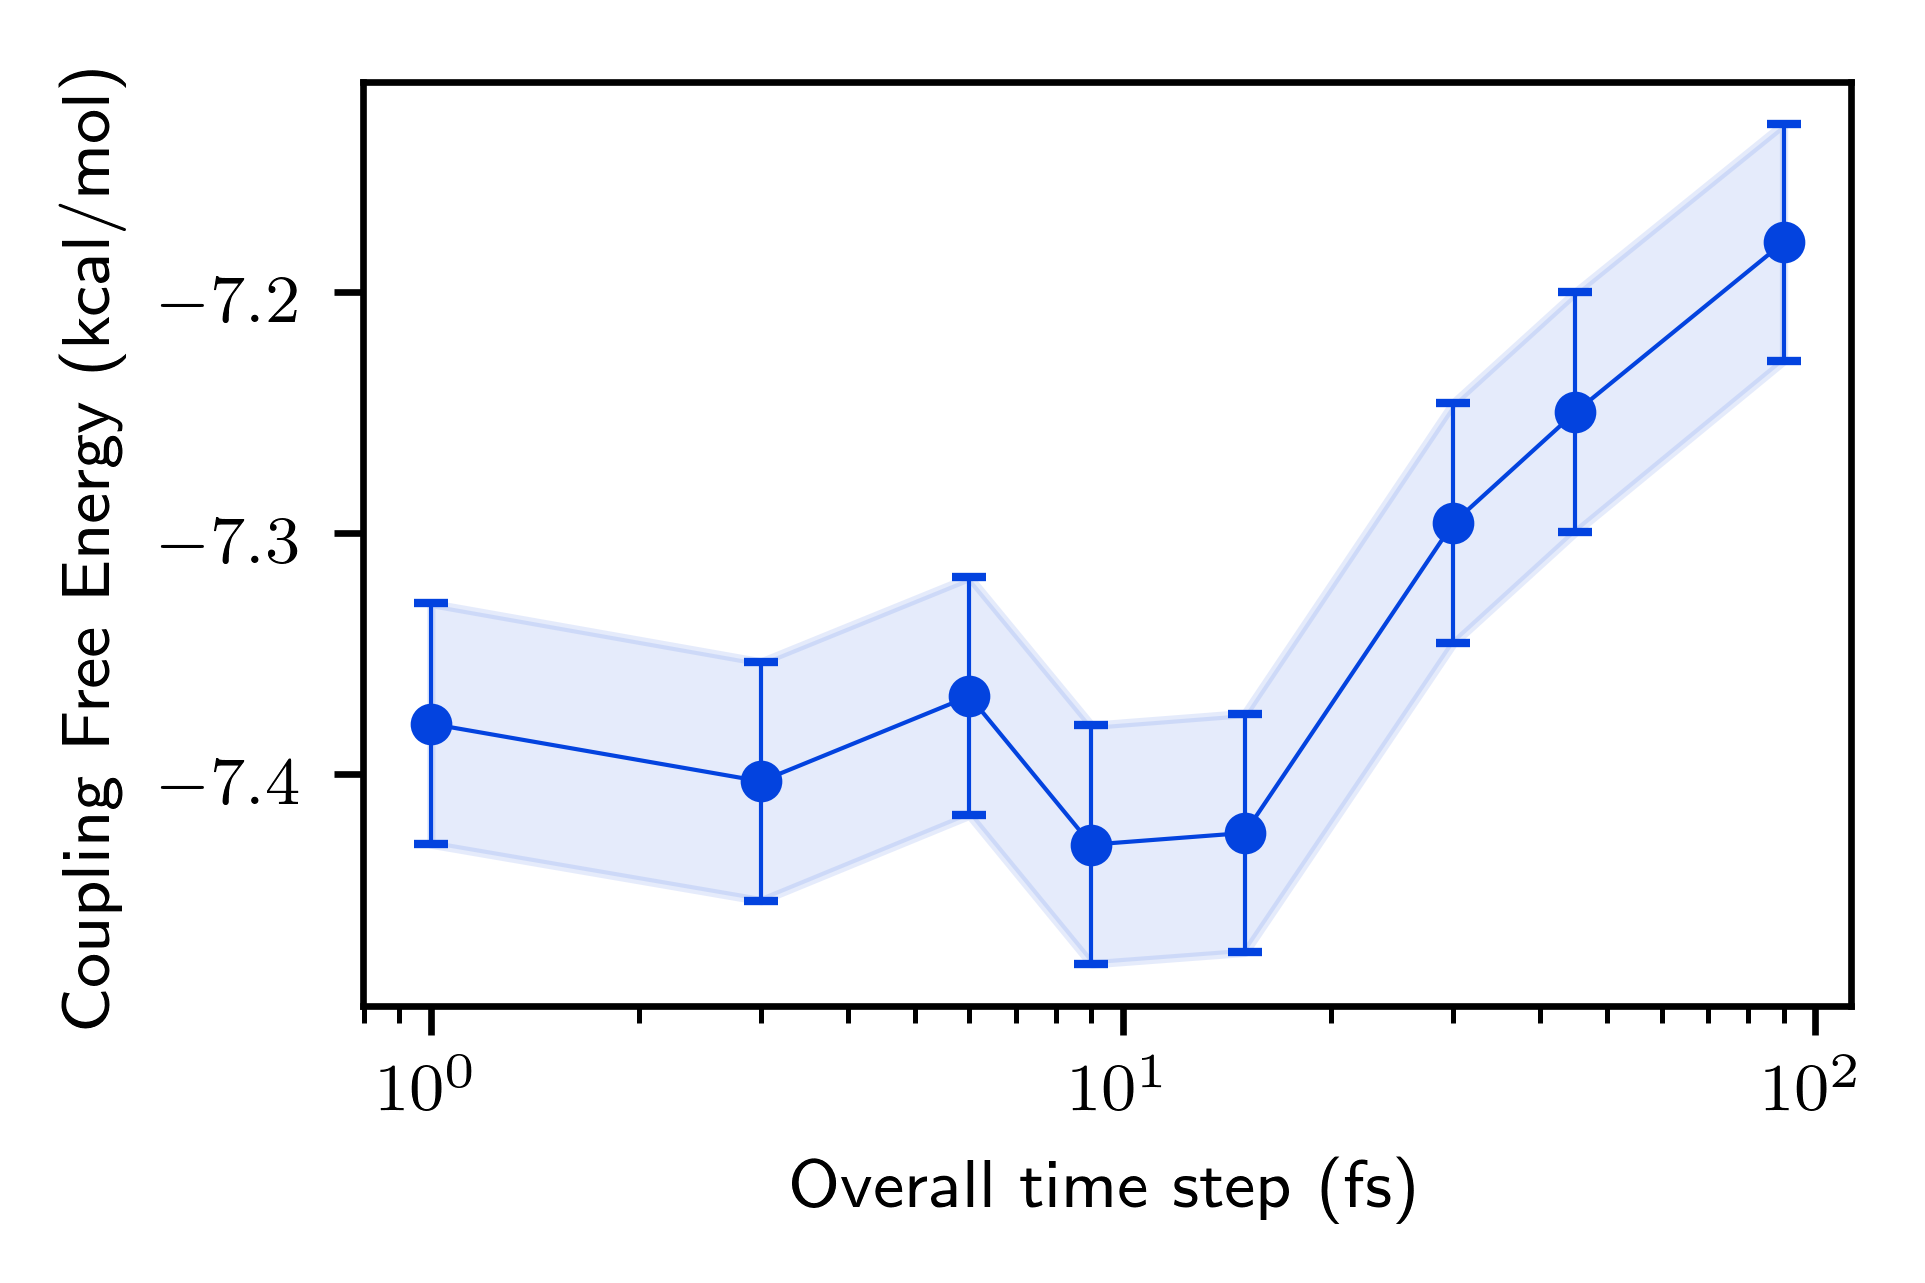
\includegraphics{gaff_phenol_coul_free_energies}
	\caption{GAFF Phenol Free Energy.}
	\label{fig:phenol coulomb free energy}
\end{figure}

\begin{figure}
	\centering
	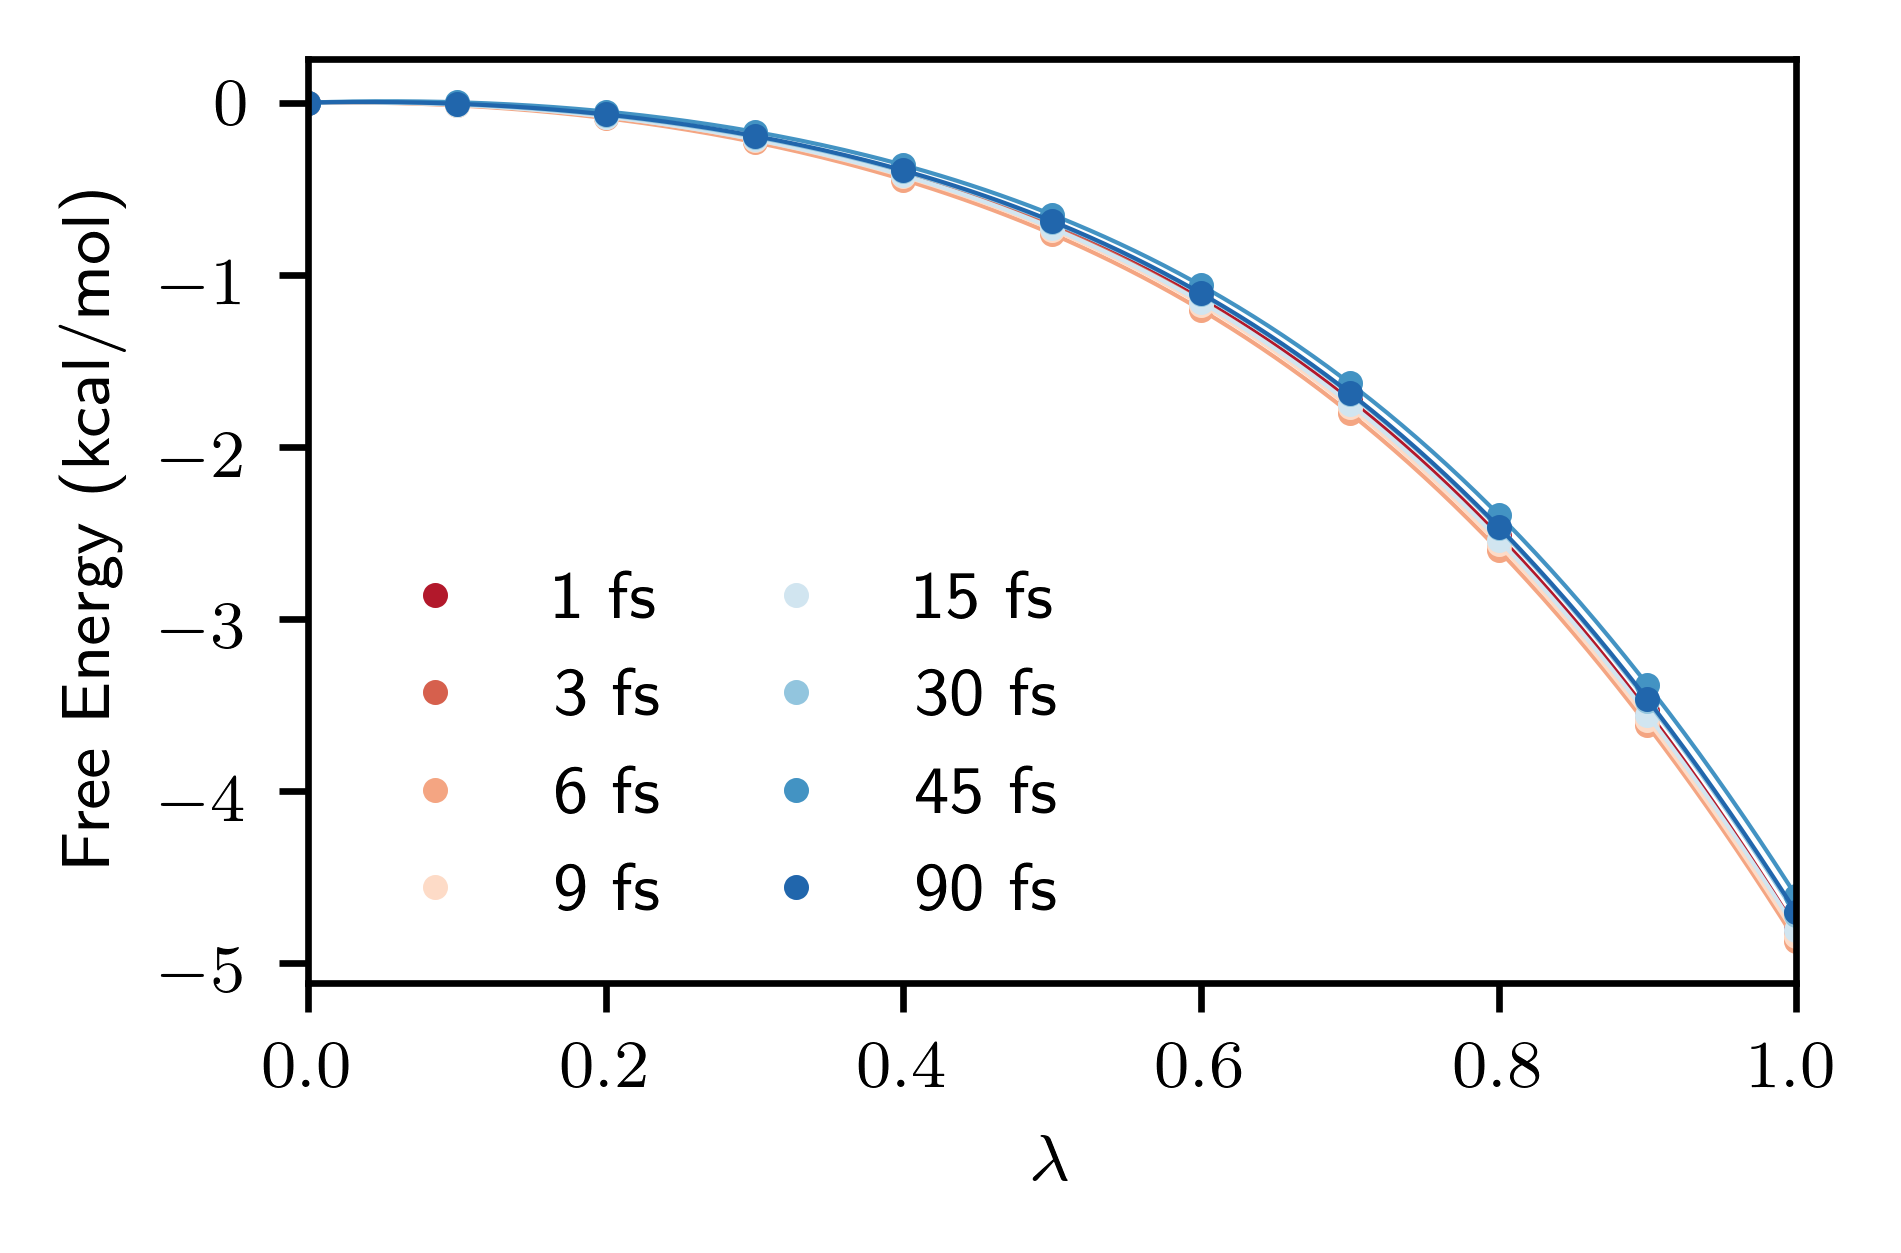
\includegraphics{gaff_dioxane_coul_free_energy_profiles}
	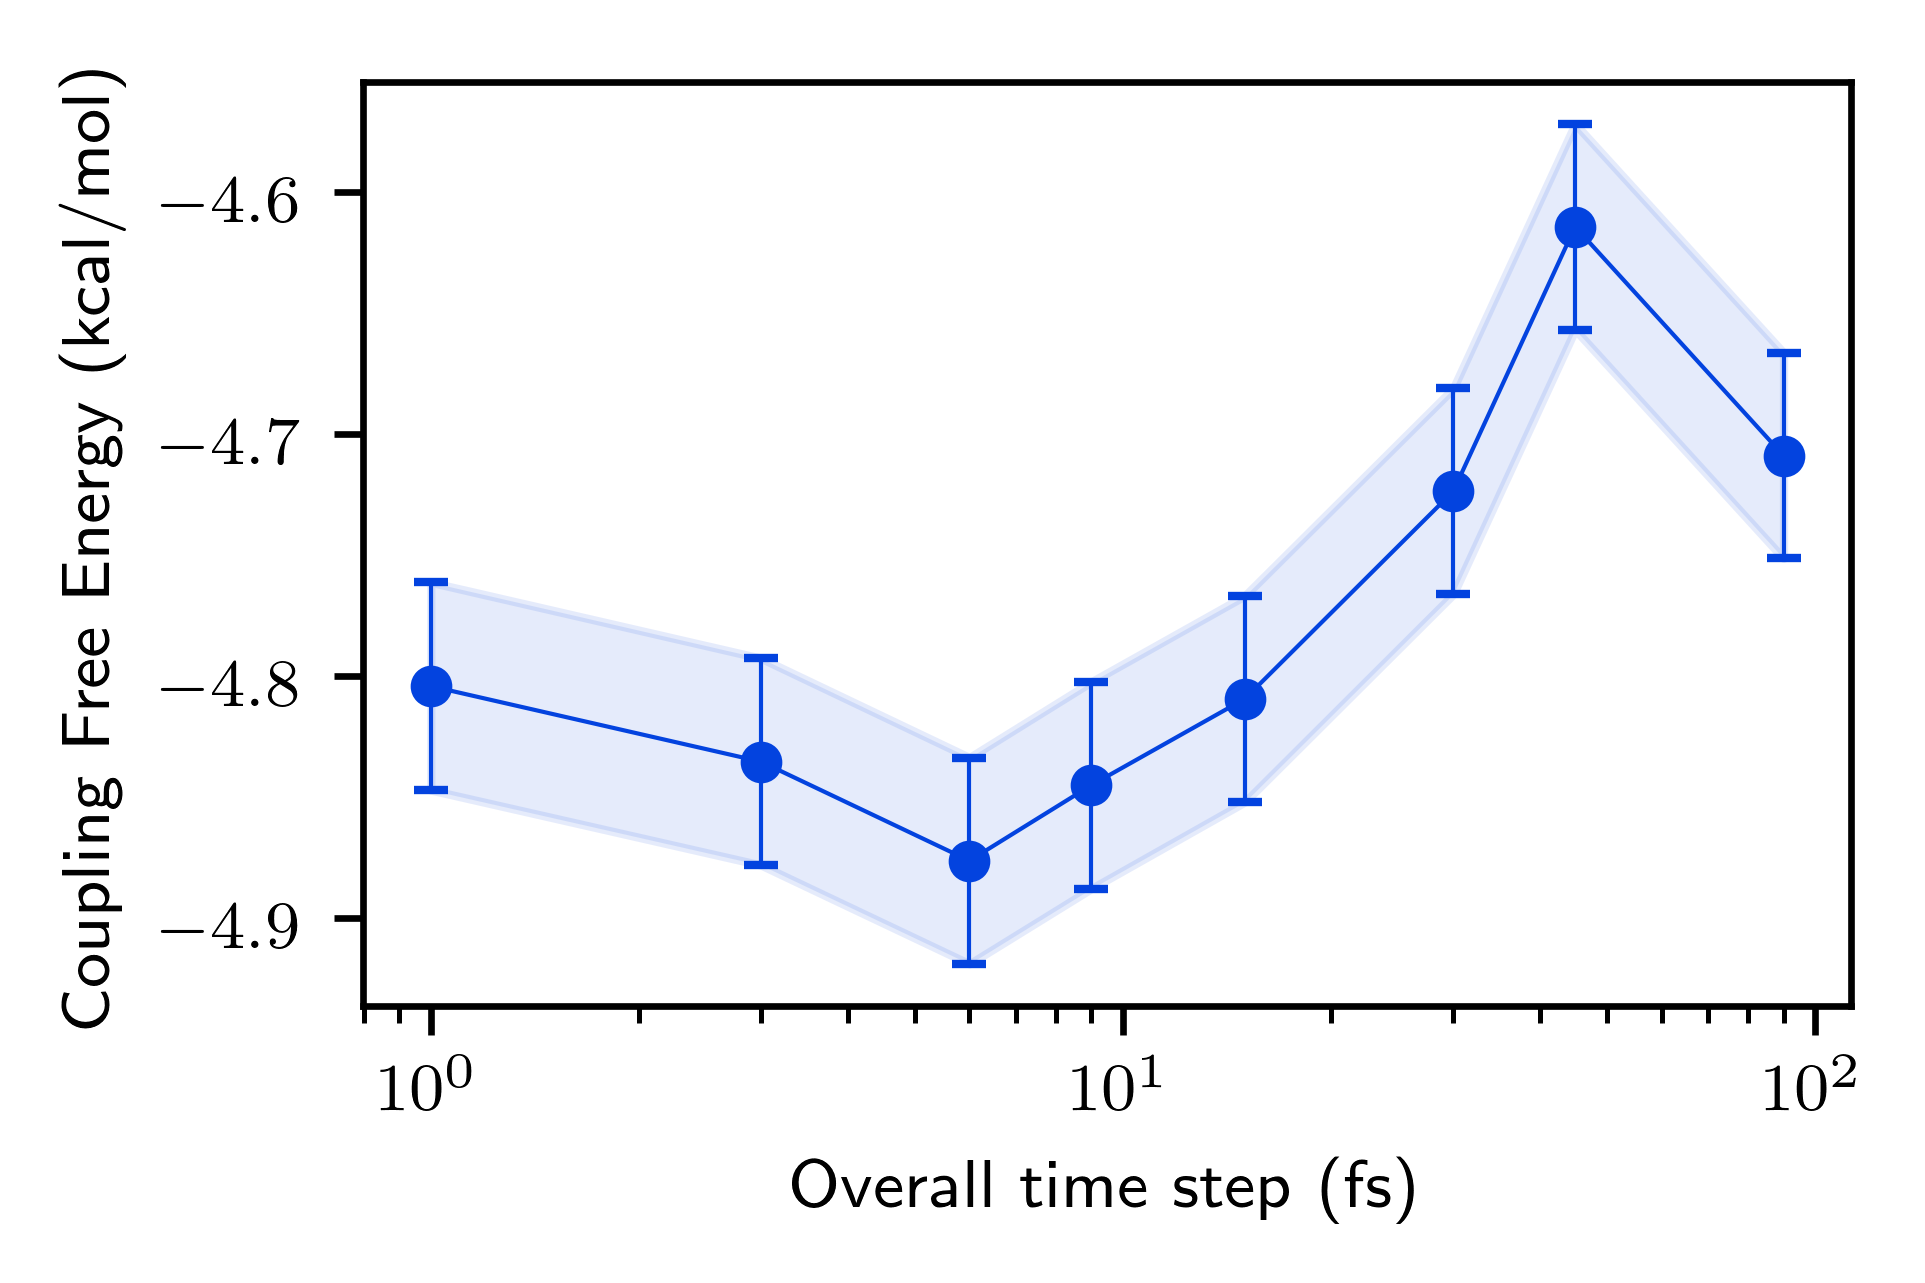
\includegraphics{gaff_dioxane_coul_free_energies}
	\caption{GAFF 1,4-dioxane Free Energy.}
	\label{fig:dioxane coulomb free energy}
\end{figure}

\begin{figure}
	\centering
	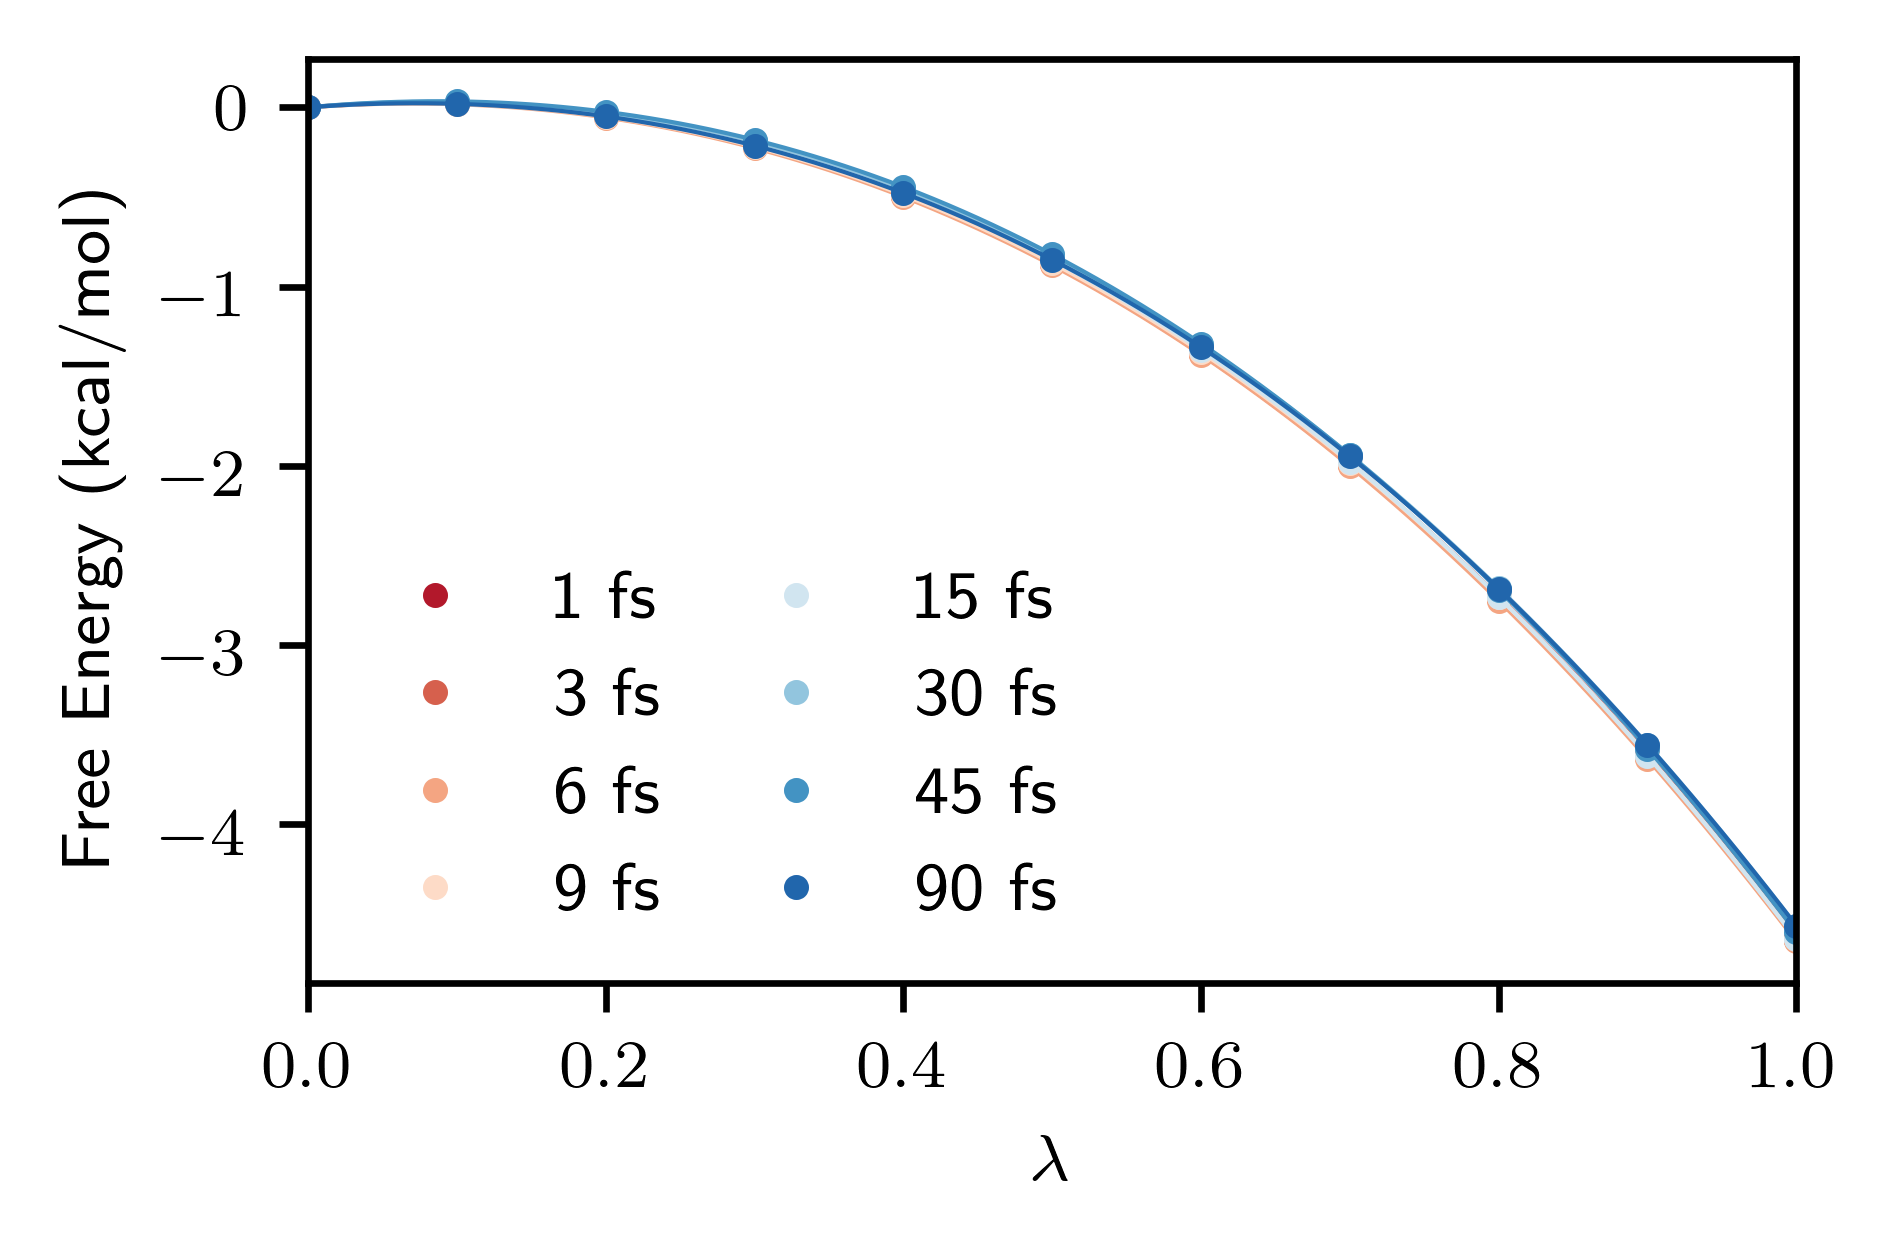
\includegraphics{gaff_dibenzo-p-dioxin_coul_free_energy_profiles}
	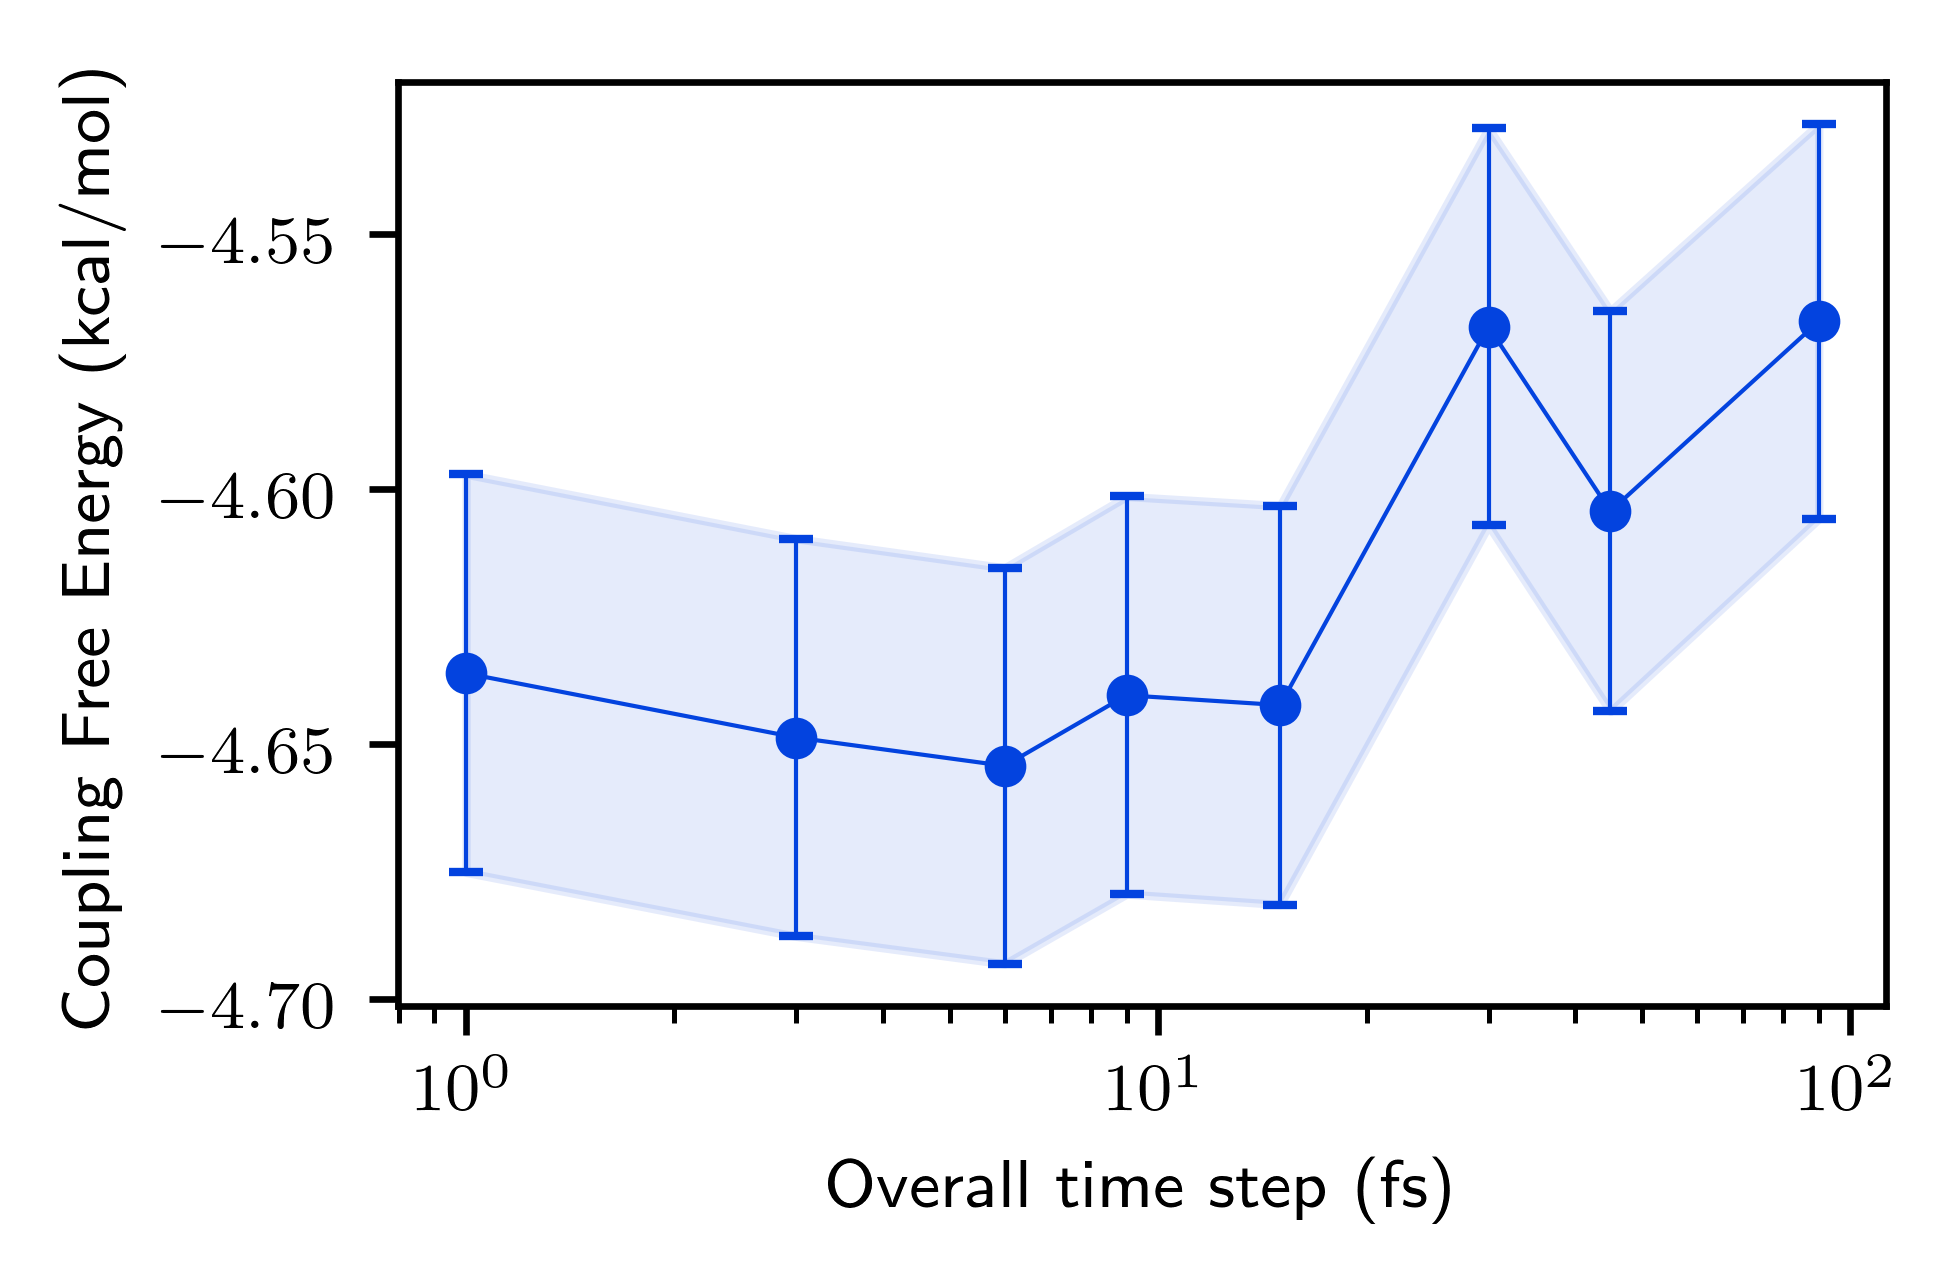
\includegraphics{gaff_dibenzo-p-dioxin_coul_free_energies}
	\caption{GAFF dibenzo-p-dioxin Free Energy.}
	\label{fig:dibenzo-p-dioxin coulomb free energy}
\end{figure}



\bibliography{solvation}

\end{document}